\cotefile{144}
\scanpage{62}
\mspage{6}

C'est ainsi que les \inserted{\unsure{cat. des}} cartes cellulaires triangulées \unsure{pondérées} \unsure{apparaissent}\deleted{\unsure{comme}} comme équivalentes à celles des \inserted{surfaces} revêtements \inserted{ramifiés} de \unsure{$\ast$} $\mathbb P^1(\mathbb C)$, ramifiés au plus en les points $0,1,\infty$. Ces revêtements sont de façon canonique des courbes algébriques (propres et lisses) sur $\mathbb C$, et la \deleted{carte} \inserted{donnée $K$ sur $X$} est l'image inverse de \inserted{l'équateur} $\mathbb P^1(\mathbb R)$, les sommets du type $i$ \deleted{sont} \inserted{forment} la fibre de $X$ au dessus du point $i\in\{0,1,\infty\}\subset\mathbb P^1(\mathbb C)$, les ordres réduits des sommets sont les \unsure{pts} de ramification; les arêtes sont les \unsure{comp.} connexes des images inverses des segments ouverts $]1,\infty[$, $]\infty,0[$, $]0,1[$.

Le cas des \inserted{(subdivision barycentrique des)} cartes ordinaires est celui où on a
\[
\rho_1^2=1,
\]
cette dernière se récupère en termes du revêtement en prenant l'image inverse du segment $[0,1]\subset U_{0,3}\subset\mathbb C$, les sommets (ordinaires) sont les pts au dessus de $0$, tandis que les points au dessus de $1$ (resp. $\infty$) sont par définition les centres des arêtes resp. centres des faces. On trouve la carte \inserted{orientée} ``universelle'' \deleted{orientée} sur $\mathbb P^1(\mathbb C)$, comme \deleted{le segment},
\[
S_0=\{0\}\subset K_\infty=[0,1]
\]
\margin{\unsure{$\ast$} (21)}
\margin{61}
\scanpage{63}
dont la subdivision barycentrique, donnée par
\[
\text{(22)}\qquad
\left\{\begin{aligned}
&S_1=\{1\},\quad S_\infty=\{\infty\},\quad K=\mathbb P^1(\mathbb R)=K_0\cup K_1\cup K_\infty\\
&\text{avec}\qquad K_0=[1,\infty],\quad K_1^{\unsure{\prime|!}}=[\infty,0],\quad
\underbrace{K_\infty=[0,1]}_{\substack{\text{comme avant}\\\text{cf (21)}}}
\end{aligned}\right.
\]
\figure{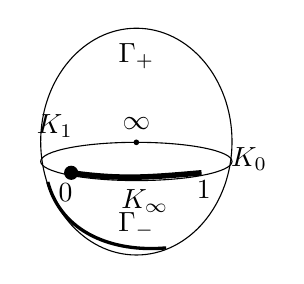
\begin{tikzpicture}[scale=.9]
\draw (0,0) ellipse (1.35 and 1.6);
\draw (0,-.28) ellipse (1.35 and .27);
\draw[line width=2pt] (-.92,-.44) to[out=-8,in=185] (.92,-.44);
\fill (-.92,-.44) circle (.1); \fill (0,-.01) circle (.04);
\node at (-1,-.72) {$0$}; \node at (.95,-.67) {$1$};
\node[above] at (0,.03) {$\infty$};
\node at (0,1.2) {$\Gamma_+$}; \node at (0,-1.18) {$\Gamma_-$};
\node at (-1.15,.22) {$K_1$}; \node at (1.59,-.24) {$K_0$};
\node at (.12,-.84) {$K_\infty$};
\draw[very thick] (-1.25,-.57) to[out=-75,in=185] (.42,-1.5);
\end{tikzpicture}}

joue le rôle de la carte orientée triangulée pondérée universelle, avec $K_0,K_1,K_\infty$ comme arêtes de types $0,1,\infty$ respectivement. Les deux \deleted{faces} \inserted{drapeaux-repères} dans la situation universelle orientée triangulée pondérée sont l'hémisphère nord $\Gamma_+$ et l'hémisphère sud $\Gamma_-$, qui apparaissent comme des ``simplexes'' topologiques, ayant mêmes sommets $0,1,\infty$, et mêmes arêtes $K_0,K_1,K_\infty$ opposées à ceux-ci. Quant aux faces de la situation initiale (21), il y en a une seule, découpe de la sphère $\mathbb P^1(\mathbb C)$ suivant le segment $K_\infty=[0,1]$, avec \deleted{une} \inserted{comme bord l'}\deleted{arête} arête unique $0'(\frac12)_-1'(\frac12)_+0'$ \deleted{qui est} qui est une boucle fermée ayant comme seul sommet $0'\mapsto0$, avec comme ``milieu'' le point $1'\mapsto1$,

\figure{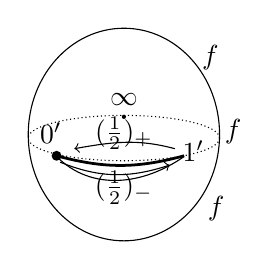
\begin{tikzpicture}[scale=.9]
\draw (0,0) ellipse (1.35 and 1.5);
\draw[densely dotted] (0,-.05) ellipse (1.35 and .32);
\draw[line width=1pt] (-.95,-.3) to[out=-15,in=195] (.85,-.3);
\draw (-.95,-.31) to[out=-45,in=215] (.85,-.31);
\draw[->] (-.9,-.39) to[out=-22,in=198] (.65,-.43);
\draw[->] (.72,-.2) to[out=165,in=10] (-.7,-.2);
\fill (-.95,-.3) circle (.07);
\fill (0,.25) circle (.03);
\node[above] at (0,.27) {$\infty$};
\node at (-1.03,.02) {$0'$};
\node at (.98,-.24) {$1'$};
\node at (0,.02) {$(\frac12)_+$};
\node at (0,-.75) {$(\frac12)_-$};
\node at (1.22,1.08) {$f$}; \node at (1.54,.04) {$f$}; \node at (1.3,-1.04) {$f$};
\end{tikzpicture}}
\margin{L'orientation marquée sur le bord de la découpe est celle induite par l'unique face $f$, avec son orientation habituelle de $\mathbb P^1(\mathbb C)$.}

les deux arcs joignant $0'$ à $1'$ sur le bord de la découpe étant ceux qui passent par $\Gamma_-$ (contenant $(\frac12)_-$) et $\Gamma_+$ (contenant $\unsure{\Gamma_+}$) respectivement. Vu depuis $\infty$, centre de l'unique face, en écartant les deux bords de la découpe, \deleted{\unsure{on en trouve donc cette}}\inserted{celle-ci apparaît} donc comme un disque de centre $\infty$, découpée par les deux rayons \deleted{$(0',\infty)$} $(\infty,0')$ et $(\infty,1')$, joignant $\infty$ à $0\sim0'$ et à $1\sim1'$ respectivement, en les deux repères $\Gamma_+$ et $\Gamma_-$ de la subdivision barycentrique, $\Gamma_+$ ayant \deleted{\unsure{son}} \deleted{\unsure{propre}}\inserted{comme} orientation propre celle induite par $f$, \deleted{\unsure{où}} et $\Gamma_-$ ayant comme orientation propre \uline{l'orientation opposée} de celle induite par $f$. \deleted{\unsure{Une}} \unsure{Par la}

\figure{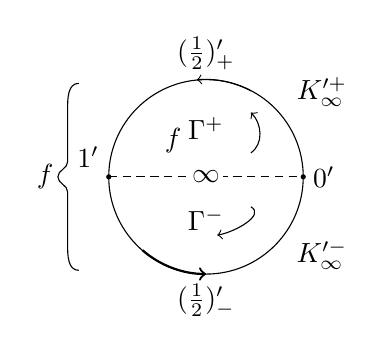
\begin{tikzpicture}[scale=.95]
\draw (0,0) circle (1.3);
\draw[densely dashed] (-1.3,0)--(1.3,0);
\fill (-1.3,0) circle (.035); \fill (1.3,0) circle (.035);
\node[above left] at (-1.3,0) {$1'$}; \node[right] at (1.3,0) {$0'$};
\node[fill=white,inner sep=1pt] at (0,0) {$\infty$};
\node at (0,.65) {$\Gamma^+$}; \node at (0,-.57) {$\Gamma^-$};
\node at (-.44,.48) {\deleted{$f$}};
\draw[->] (.6,.32) to[out=35,in=-45] (.6,.86);
\draw[->] (.6,-.4) to[out=-30,in=10] (.15,-.78);
\draw[->] (.6,1.15) arc (62:95:1.3);
\draw[->,thick] (-.85,-.98) arc (229:270:1.3);
\node[above] at (0,1.3) {$(\frac12)'_+$};
\node[below] at (0,-1.3) {$(\frac12)'_-$};
\node at (1.55,1.13) {$K_\infty^{\prime+}$};
\node at (1.55,-1.05) {$K_\infty^{\prime-}$};
\draw (-1.7,1.25) to[out=180,in=90] (-1.85,.9)--(-1.85,.2)
to[out=-90,in=90] (-1.98,0) to[out=-90,in=90] (-1.85,-.2)--(-1.85,-.9)
to[out=-90,in=180] (-1.7,-1.25);
\node at (-2.15,0) {$f$};
\end{tikzpicture}}
\margin{Attention, si on place $\Gamma^+$ au dessus de l'``équateur'' $0'\infty1'$, $0'$ doit être placé à droite de $\infty$, $1'$ à gauche !}
\margin{62}
\scanpage{64}
\mspage{7}
théorie de la représentation conforme, ce disque holomorphe doit être isomorphe au disque \unsure{standart} $\mathbb D$, via un isomorphisme unique
\[
g:\mathbb D\xrightarrow{\sim}f\qquad
\begin{aligned}
0&\longmapsto\infty\quad\text{(centre de $f$)}\\
1&\longmapsto0'\quad\text{(unique sommet de $f$)}
\end{aligned}
\]
\figure{\begin{tikzpicture}
\draw (0,0) circle (1.25);
\draw[->,thick] (1.17,.44) arc (20:60:1.25);
\fill (0,0) circle (.025); \node[below] at (0,0) {$0$};
\fill (1.25,0) circle (.06); \node[right] at (1.25,0) {$1$};
\fill (-1.25,0) circle (.025); \node[left] at (-1.25,0) {$-1$};
\fill (0,1.25) circle (.025); \node[above] at (0,1.25) {$i$};
\fill (0,-1.25) circle (.025); \node[below] at (0,-1.25) {$-i$};
\end{tikzpicture}}
et on s'attend que l'on ait de plus
\[
\left\{\begin{aligned}
g(-1)&=1'\\
g(i)&=(\tfrac12)'_+\\
g(-i)&=(\tfrac12)'_-
\end{aligned}\right.
\]

Comment trouver $g$ ? On \deleted{trouve}\inserted{voit} que le disque $\mathbb D$ est l'hémisphère positif du \unsure{le} ``monogone'' \unsure{standart} $X_1$\inserted{$=\mathbb P^1(\mathbb C)$}, qui \deleted{\unsure{est}} a comme seul sommet $1$, comme seule arête l'équateur $\mathbb P^1(\mathbb R)$, comme centres des \inserted{deux} faces $0$ et $\infty$ (qui forment l'axe polaire), comme milieu d'arête $-1$.
\figure{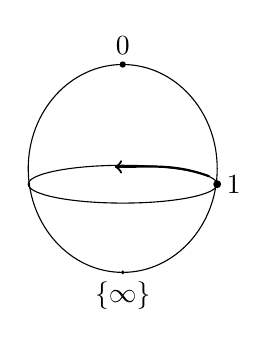
\begin{tikzpicture}
\draw (0,0) ellipse (1.2 and 1.32);
\draw (0,-.2) ellipse (1.2 and .24);
\draw[->,thick] (1.1,-.1) to[out=160,in=0] (-.1,.02);
\fill (0,1.32) circle (.04); \node[above] at (0,1.32) {$0$};
\fill (1.2,-.2) circle (.05); \node[right] at (1.2,-.2) {$1$};
\fill (0,-1.32) circle (.025); \node[below] at (0,-1.32) {$\unsure{\{\infty\}}$};
\end{tikzpicture}}
\deleted{\unsure{Il}}\inserted{Alors $X_1$} est un revêtement d'ordre $2$ de $X_0$\inserted{$=\mathbb P^1(\mathbb C)$}, ramifié \deleted{en dehors} au plus en $\{0,1,\infty\}$, (l'ordre du revêtement est le nb de repères \inserted{directs}, qui est $2$) avec
\[
\deleted{\unsure{\infty\longmapsto}}\qquad
g:\quad\begin{aligned}
1&\longmapsto0\\
-1&\longmapsto1\\
0,\infty&\longmapsto\infty
\end{aligned}
\]
ce qui épuise les fibres en $0,1,\infty$, et montre que la ramification est $2$ sur $0,1$, et pas de ramification sur $\infty$. \deleted{\unsure{Si l'on a}}\inserted{Pour} \unsure{avoir} la \deleted{\unsure{m}} situation analogue, \inserted{$g':\mathbb P^1(\mathbb C)\mathbin{-}\mathbb P^1(\mathbb C)$} mais avec
\[
g':\quad\begin{aligned}
0&\longmapsto0\\
\infty&\unsure{\longmapsto|\mathbin{-}}\infty\\
1,-1&\longmapsto1
\end{aligned}
\]
on aurait évidemment
\[
g'(z)=z^2,
\]
\margin{63}
\scanpage{65}
\mspage{8}
et on a
\[
g(z)=\varphi g'(\psi(z))
\]
où $\varphi,\psi$ sont les transformations homographiques satisfaisant
\[
\psi:\left\{\begin{array}{c}1\\-1\\0,\infty\end{array}\right.
\longrightarrow
\left\{\begin{array}{c}0\\\infty\\1,-1\end{array}\right.
\qquad
\varphi:\left\{\begin{array}{cc}0&0\\\infty&1\\1&\infty\end{array}\right.
\]
donc \deleted{$\unsure{\varphi}$}
\[
\psi(z)=\frac{z-1}{z+1}\qquad
\varphi(z)=\sigma_0(z)=\frac{z}{z-1}
\]
d'où
\[
g(z)=\frac{\left(\frac{z-1}{z+1}\right)^2}{\left(\frac{z-1}{z+1}\right)^2+1}
=\frac{(z-1)^2}{(z-1)^2-(z+1)^2}
=\frac{(z-1)^2}{-4z}
\]
\[
\text{(23)}\qquad g(z)=-\frac1{4z}(z-1)^2
\]
réalise l'isomorphisme conforme du disque unité $\mathbb D$ sur la découpe $f$ de $\mathbb P^1(\mathbb C)$ suivant $[0,1]$, avec les valeurs annoncées plus haut...
\[
\text{---}
\]

Le groupe $\Pi_{0,3}^{\tau}$ apparaît comme groupe fondamental mixte
\[
\text{(24)}\qquad
\Pi_{0,3}^{\tau}\simeq\Pi_1(U_{0,3},\{1,\tau\};P_+)
\]
\margin{\uline{NB} \unsure{Ici}\quad
$\rho_i=\lambda_{i+1}^{\deleted{\unsure{-1}}}\lambda_{i-1}^{-1}$}

Introduisant les chemins \inserted{$\lambda_i\ (i\in\{0,1,\infty\})$} de $P_-$ à $P_+$, formés des demi-arcs de grand cercle passant par les $Q_i$ (\inserted{$Q_i$,} milieux des arcs de grand cercle joignant $j$ à $k$, où $\{i,j,k\}=\{0,1,\infty\}$), on aura, en tant que flèches de $\Pi_1(U_{0,3},\{1,\tau\})$ :
\[
\tau_i=\left(\underbrace{\lambda_i}_{\tau P_+=P_-\to P_+},
\underset{\substack{\unsure{\uparrow}\\\{1,\tau\}}}{\tau}\right)
\]
\figure{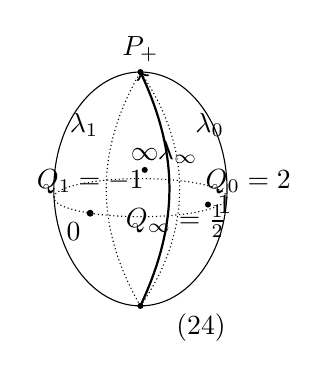
\begin{tikzpicture}[scale=1.1]
\draw (0,0) ellipse (1 and 1.35);
\draw[densely dotted] (0,-.1) ellipse (1 and .22);
\draw[densely dotted] (0,-1.35) to[out=120,in=-120] (0,1.35);
\draw[densely dotted] (0,-1.35) to[out=55,in=-55] (0,1.35);
\draw[thick,->] (0,-1.35) to[out=65,in=-65] (0,1.35);
\fill (0,1.35) circle (.035); \node[above] at (0,1.35) {$P_+$};
\fill (0,-1.35) circle (.035);
\fill (-.58,-.28) circle (.04); \node[below left] at (-.58,-.28) {$0$};
\fill (.78,-.18) circle (.035); \node[right] at (.78,-.18) {$1$};
\fill (.05,.22) circle (.035); \node[above] at (.05,.22) {$\infty$};
\node at (-.65,.74) {$\lambda_1$}; \node at (.8,.74) {$\lambda_0$};
\node at (.43,.43) {$\lambda_\infty$};
\node at (-.58,.08) {$Q_1=-1$}; \node[right] at (.64,.08) {$Q_0=2$};
\node at (.41,-.37) {$Q_\infty=\frac12$};
\node at (.7,-1.6) {(24)};
\end{tikzpicture}}
\margin{64}
\scanpage{66}
Cette interprétation montre que la catégorie \inserted{isotopique} des cartes (triangulées) pondérées (de type $\{0,1,\infty\}$) est équivalente à \inserted{(une ss-cat. pleine de)} celle des \inserted{$\{1,\tau\}$-}revêtements \inserted{finis} étales de $U_{0,3}$, \deleted{tels que}\inserted{disons ceux} satisfaisant à une condition supplémentaire (savoir que sur l'ens. à op. correspondant, $\tau_0,\tau_1,\tau_\infty$ opèrent sans pts fixes). Mais on vérifie, $\unsure{\Longleftrightarrow}$ de suite que \deleted{\unsure{pour le}} pour un $\{1,\tau\}$ revêtement de $U_{0,3}$, les points fixes des $\tau_i$ correspondants correspondent aux composantes connexes de $U^\tau$ qui sont au dessus de l'arc de $U_{0,3}(\mathbb R)$ opposé à $P_i$ i.e \deleted{\unsure{au b}} de centre $Q_i$ -- donc la condition signifie que \deleted{$\unsure{U^\tau=\varnothing}$} l'on a
\[
\text{(25)}\qquad U^{\prime\tau}=\varnothing\quad\text{i.e.}\quad X^{\prime\tau}=\varnothing
\]
où $X'$ est le revêtement ramifié de $\mathbb P^1(\mathbb C)$ qui prolonge $U'$. [NB \deleted{\unsure{si on avait}} a priori $X^{\prime\tau}$ est une courbe analytique réelle \deleted{plongée}\inserted{contenue} dans $X'$; \deleted{\unsure{qui} $X^{\prime\tau}$} est \inserted{donc} vide dès que sa trace sur $U'=X'\smallsetminus\unsure{\text{ens fini}}$ \deleted{(ens fini)} l'est.)] \inserted{NB.} En termes de la carte pondérée initiale, $X'$ est le revêtement de ses orientations \inserted{locales}, $\tau_{X'}$ \deleted{\unsure{en}} l'autom. \unsure{d'ordre} \unsure{passant} à l'orientation opposée..., qui en effet doit être sans points fixes).

Indépendamment de la condition restrictive (25), la donnée du $\{1,\tau\}$ revêtement \inserted{ramifié} de $\unsure{\boldsymbol{\Sigma}|\Sigma}=\mathbb P^1(\mathbb C)$,
\margin{65}
\scanpage{67}
\mspage{9}
étale au dessus de \inserted{$\overline\Sigma^*=$} $U_{0,3}$, \deleted{revient à}\inserted{i.e.} la donnée d'un revêtement ramifié de $\Sigma$ étale au dessus de $U_{0,3}$, plus une op. de $\{1,\tau\}$ dessus compatible avec l'opération sur $\Sigma$, revient à la donnée d'une \uline{donnée de descente} de $\mathbb C$ à $\mathbb R$ dans un revêtement ramifié, étale sur $U_{0,3\,\mathbb C}$, du \deleted{$\unsure{\Sigma}$}\inserted{$\mathbb C$-}schéma $\Sigma_{\mathbb C}$. Donc la catégorie de ces revêtements mixtes \inserted{est} équivalente à celle des revêtements ramifiés du schéma \deleted{$U_{0,3}$}\inserted{$\Sigma_{\mathbb R}=\mathbb P^1_{\mathbb R}$}, étales au dessus de $\deleted{U_{0,3}}{}_{\mathbb R}=\overline\Sigma_{\mathbb R}^*=\Sigma_{\mathbb R}\smallsetminus\{0,1,\infty\}$. On trouve ainsi un \uline{foncteur pl. fidèle} canonique
\diagram{\begin{tikzcd}[ampersand replacement=\&,column sep=large]
\begin{gathered}
\text{(26)}\quad\text{cartes triangulées pondérées}\\
\inserted{\text{finies}}\\
\text{de type }\{0,1,\infty\}
\end{gathered}
\arrow[r, "\unsure{\colon}" description]
\&
\begin{gathered}
\text{revêtements }\inserted{\text{finis}}\text{ étales}\\
\text{du schéma }\mathbb P^1_{\mathbb R}\smallsetminus\{0,1,\infty\}\\
(\simeq\text{ rev. ramifiés de}\\
\mathbb P^1_{\mathbb R},\ \text{étales au dessus}\\
\text{de }U_{03\,\mathbb R}^{\unsure{\circ|*}}=\mathbb P^1_{\mathbb R}\smallsetminus\{0,1,\infty\}
\end{gathered}
\end{tikzcd}}

L'image essentielle est formée des rev. $X'$ tels que \deleted{$\unsure{X'(\mathbb R)=}$}
\[
\text{(27)}\qquad X'(\mathbb R)=\varnothing
\]
interprétation qui ne fait que traduire (25) puisque
\[
X'(\mathbb R)=\underbrace{X'(\mathbb C)}_{\substack{\text{noté }X'\\\text{dans (25)}}}^{\tau}.
\]
Le foncteur en sens inverse est donné en associant à tt rev. \inserted{ramifié} $X'$ de $\mathbf X$, étale sur $U_{0,3}$, \unsure{l'esp. top.|l'ens. top.} $X'(\mathbb C)$, muni de l'image inverse $\left.X'(\mathbb C)\right|_{(\mathbb P^1_{\mathbb R}=\overline\Sigma_{\mathbb R})}$ de l'ens. des pts réels de $\mathbb P^1(\mathbb C)=\overline\Sigma$,
\margin{66}
\scanpage{68}
\margin{\deleted{(\unsure{B4 B64})}}
qui définit une triangulation (orientée) avec pondération par les images inverses des pts $0,1,\infty$ (qui forment \inserted{\deleted{par définition}} une partition de l'ens des sommets $\unsure{\}}$ de la triangulation, défini comme l'ens des pts au dessus de $\{0,1,\infty\}$), et en passant au quotient par la conjugaison complexe -- ce qui donne une surface sans bord, grâce à la condition (27). Dans le cas où on ne pose pas cette condition, l'espace quotient
\[
\text{(28)}\qquad X=X'(\mathbb C)/\tau
\]
est une surface à bord compacte (et munie d'une structure conforme...), et on pourrait étendre \inserted{(de façon ess.t unique)} la définition des cartes \inserted{\deleted{finies}} triangulées pondérées sur des surfaces compactes \unsure{à} bord, au cas des surfaces compactes à bord, de telle façon que (26) devienne une équivalence de \uline{catégories}.
\figure{\begin{tikzpicture}\draw (0,0)--(.28,-.38);\end{tikzpicture}}

\textcircled{4.} On peut introduire, sur nos cartes (orientée ou non), des conditions de la forme
\[
\text{(29)}\qquad \rho_i^{\nu_i}=1
\]
\deleted{\unsure{type}} où $\nu_i\in\unsure{\overline{\mathbb N}^{*}|\mathbb N^{*}}$, qui signifie donc que
\margin{67}
\scanpage{69}
\margin{68}
\mspage{10}
dans la carte triangulée pondérée envisagée, les sommets de type $i$ \deleted{sont d'}\inserted{ont un} ordre réduit \uline{divisant} $\nu_i$. Une telle condition peut être introduite pour un ou plusieurs indices $i$. Dans le cas des cartes ordinaires (interprétées comme définissant une triangulation pondérée, via la subdivision barycentrique) une relation
\[
\text{(30)}\qquad \rho_0^{\nu_0}=1\qquad(\text{resp. }\rho_\infty^{\nu_\infty}=1)
\]
signifie que les sommets sont d'ordre divisant $\nu_0$ (resp. que les faces sont d'ordre divisant $\nu_\infty$).

Quant à la relation
\[
\text{\deleted{\unsure{(31)}}\unsure{(*)}}\qquad \rho_1^{\nu_1}=1,
\]
comme on a déjà $\rho_1^2=1$, ou bien $\nu_1$ est \inserted{pair} et cette relation$^{\unsure{(*)}}$ est automatiquement satisfaite, ou bien $\nu_1$ est impair, et elle implique
\[
\rho_1=1
\]
ce qui signifie que la carte correspond à un revêtement de $\mathbb P^1_{\mathbb C}$ ramifié seulement en $0$ et $\infty$, donc à un revêtement ``cyclotomique'' $z\mapsto z^n$ ($n\in\mathbb N$), \deleted{cas qui} donnant lieu à \deleted{des} cartes régulières \inserted{sphériques} de groupe $\mathbb Z/n\mathbb Z\simeq\mu_n(\mathbb C)$ ayant un seul sommet, une seule face, et $n$ arêtes disposées circulairement (carte isomorphe à sa duale, visiblement) -- ce qui est relativement trivial. Donc on peut dire
\figure{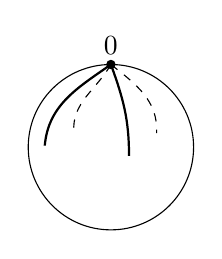
\begin{tikzpicture}
\draw (0,0) circle (1.05);
\fill (0,1.05) circle (.06); \node[above] at (0,1.05) {$0$};
\draw[thick] (0,1.05) to[out=-145,in=85] (-.84,.02);
\draw[thick] (0,1.05) to[out=-70,in=90] (.23,-.11);
\draw[dashed] (0,1.05) to[out=-120,in=95] (-.47,.18);
\draw[dashed] (0,1.05) to[out=-38,in=87] (.58,.18);
\end{tikzpicture}}
\scanpage{70}
que dans le cas des cartes ordinaires, les relations intéressantes à considérer sont du type (30), à l'exclusion de $\unsure{(*)}$. \figure{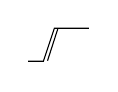
\begin{tikzpicture}[baseline=-.2ex,scale=.35]
\draw (0,0)--(.55,0)--(.95,1.2)--(2.2,1.2);
\draw (.7,.02)--(1.08,1.2);
\end{tikzpicture}} On considère que l'on a \deleted{\unsure{les arêtes}}\inserted{$\rho_i^\infty=1$} par définition, de sorte que l'on peut considérer un système de conditions (29), où pour tt $i\in\{0,1,\infty\}$, on a
\[
\text{(31)}\qquad \nu_i\in\overline{\mathbb N}^{*}=\mathbb N^{*}\cup\{+\infty\}.
\]

Les cartes (finies) pondérées triangulées correspondantes sont déterminées à l'aide du groupe quotient
\[
\text{(32)}\qquad
\Pi_{0,3}/\langle\rho_0^{\nu_0},\rho_1^{\nu_1},\rho_\infty^{\nu_\infty}\rangle
\qquad\text{(cas orienté)}
\]
ou par le quotient
\[
\text{(32 bis)}\qquad
\Pi_{0,3}^{\tau}/\langle\rho_0^{\nu_0},\rho_1^{\nu_1},\rho_\infty^{\nu_\infty}\rangle
\qquad\text{(cas non orienté)}
\]
qui s'identifie à une extension de $\{1,\tau\}$ par (32). Ce dernier groupe s'interprète comme groupe fondamental ``avec signature''
\[
\text{(33)}\qquad
\Pi_{0,3}/\langle(\rho_i^{\nu_i})\rangle
\simeq\Pi_1(\mathbb P^1(\mathbb C),\nu_*;P_+)
\]
\[
\nu_*=(\nu_0\unsure{R_0|P_0}+\nu_1\unsure{R_1|P_1}+\nu_\infty\unsure{R_\infty|P_\infty})
\quad\text{signature sur }\mathbb P^1_{\mathbb C}
\]
ou encore comme groupe fondamental de la multiplicité (topologique, analytique ou schématique, au choix -- mais dans ce dernier cas il s'agit du complété profini...)
\margin{69}
\scanpage{71}
\margin{\deleted{(\unsure{2 mots})}}
\mspage{11}
\[
\text{(34)}\qquad
\mathcal X(\mathbb P^1_{\mathbb C},\nu_*)=
\deleted{\text{catégorie}}\inserted{\text{topos}}\ \text{des }\deleted{\text{espaces}}\inserted{\text{surfaces}}\ \text{topologiques (\unsure{pas}}
\]
néc. séparées) ramifiées sur $\mathbb P^1_{\mathbb C}$, avec indices de ramification, \deleted{en} les points au dessus d'un $R_i\in\operatorname{supp}\nu_*$, divisant $\nu(R_i)=\nu_i$.

\margin{\uline{NB} Ce topos est une multiplicité topologique, loc. surface topologique, elle est canoniquement orientée.}

i.e. on a un isom. canonique
\[
\text{(35)}\qquad
\Pi_{03}/\langle(\rho_i^{\nu_i})\rangle
\simeq\Pi_1(\mathbb P^1_{(\mathbb C)},\nu_*;P_+)
\overset{\text{déf}}{=}\Pi_1(\mathcal X(\mathbb P^1(\mathbb C),\nu_*),P_+),
\]
et de même
\[
\begin{aligned}
\text{(36)}\qquad
\Pi_{0,3}^{\tau}/\unsure{\langle}(\rho_i^{\nu_i})\rangle
&\simeq\Pi_1(\mathbb P^1(\mathbb C),\{1,\tau\},\nu_*;P_+)\overset{\text{déf}}{=}\\
&\Pi_1(\mathcal X(\mathbb P^1(\mathbb C),\nu_*\deleted{\unsure{\}}},\{1,\tau\}),P_+)
\end{aligned}
\]
où
\[
\text{(37)}\qquad
\mathcal X(\mathbb P^1(\mathbb C),\nu_*,\{1,\tau\})
=(\mathcal X(\mathbb P^1(\mathbb C),\nu_*),\{1,\tau\})
\]
topos mixte défini par le topos (34) avec l'opération naturelle de $\{1,\tau\}$ dessus.

\margin{\uline{NB} c'est encore une multiplicité topologique, localement une surface, mais cette multiplicité n'est pas orientable...}

Passant aux complétés profinis, on trouve
\[
\begin{aligned}
\text{(38)}\qquad
\widehat\Pi_{0,3}/\langle(\rho_i^{\nu_i})\rangle
&\simeq\Pi_1(\underbrace{\mathbb P^1_{\mathbb C}}_{\uline{\text{schéma}}},\nu_*;P_+)\\
&\simeq\Pi_1(\mathbb P^1_{\overline{\mathbb Q}},\nu_*;P_+)
\end{aligned}
\]
\[
\begin{aligned}
\text{(39)}\qquad
\widehat\Pi_{0,3}^{\tau}/\langle(\rho_i^{\nu_i})\rangle
&\simeq\Pi_1(\underbrace{\mathbb P^1_{\mathbb R}}_{\text{schéma}},\nu_*;P_+)\\
&\simeq\Pi_1(\mathbb P^1_{\overline{\mathbb Q}\cap\mathbb R},\nu_*;P_+)
\end{aligned}
\]
(et \deleted{cette} l'interprétation \inserted{(38)} montre qu'il y a une
\margin{70}
\scanpage{72}
opération extérieure de $\operatorname{Gal}(\overline{\mathbb Q}/\mathbb Q)$ sur le premier mb de (38), et en particulier sur $\widehat\Pi_{0,3}$ lui-même...).

Les cas les plus intéressants sont les \deleted{deux} suivants :

I) $\nu_0=\nu_1=\nu_\infty=+\infty$ : on retrouve $\Pi_{0,3}^{\tau}$ et $\Pi_{0,3}^{\deleted{\unsure{\tau}}}$, classifiant les cartes triangulées pondérées (resp. orientées).

II) $\nu_0=\nu_\infty=+\infty$, $\nu_1=2$ : on retrouve les groupes $\Pi_{0,3}^{\tau}/\langle\rho_1^2\rangle$ et $\Pi_{0,3}/\langle\rho_1^2\rangle$, classifiant les cartes ordinaires.

III) $\nu_0=\infty$, $\nu_1=2$, $\nu_\infty=3$ : donnent les groupes $\Pi_{0,3}^{\tau}/\langle\rho_1^2,\rho_\infty^3\rangle$ et $\Pi_{0,3}/\langle\rho_1^2,\rho_\infty^3\rangle$, classifiant les cartes ordinaires \uline{triangulées} (\uline{pas} pondérées !), i.e. dont toutes les faces sont \deleted{des monogones \unsure{ou}} d'ordre divisant $3$ i.e. sont des monogones ou des triangles -- dans le cas non orienté, et dans le cas orienté. On trouve des isomorphismes remarquables (via (35)(36))

\margin{Ces isomorphismes sont valables pour tte situation d'un groupe d'opérateurs $G$ fidèle sur une surface topol. $X$, avec groupes d'isotropie finis, \unsure{en interprétant} $\Pi_1(X,G;P)$ mixte, en termes \deleted{\unsure{topologique}} d'un groupe fondamental ``avec signature'' $(\Sigma_0)$.}

\diagram{\begin{tikzcd}[ampersand replacement=\&,column sep=large,row sep=large]
\text{(40)}\ \raisebox{-1.1cm}{$\left\{\rule{0pt}{2.8cm}\right.$}
\&
\underbrace{\Pi_{0,3}^{\tau}/\langle\rho_1^2,\rho_\infty^3\rangle}_{\text{groupes cartographiques}}
\&
\underbrace{\Pi_1(U_{0,3},\unsure{\mathcal G_3|\mathfrak S_3}\times\{1,\tau\};P_+)}_{\Pi_{0,3}^{D_3,\tau}}
\arrow[l,"\sim"']
\\
\&
\unsure{=}\ \underbrace{\Pi_{0,3}/\langle\rho_1^2,\rho_\infty^3\rangle}_{\substack{\uline{\text{triangulés}},\ \unsure{\text{non or. resp.}}\\\text{orienté}}}
\arrow[r,leftrightarrow,"\sim"]
\&
\overbrace{\Pi_1(U_{0,3},\unsure{\mathcal G_3|\mathfrak S_3};P_+)}^{\Pi_{0,3}^{D_3}}
\end{tikzcd}}
\margin{$\{\rho_1,\rho_\infty\mid\rho_1^2=\rho_\infty^3=1\}$}
\margin{71}
\scanpage{73}
\mspage{12}
dont le deuxième est donné par
\[
\text{(41)}\qquad
\boxed{\rho\longmapsto\rho_\infty^{-1},\quad\sigma_\infty\longmapsto\rho_1},
\qquad
\underset{\substack{\Vert\\\sigma_\infty\rho}}{\varepsilon_0}\longmapsto\rho_0
\]
\margin{Attention à l'exposant !}
et le \uline{premier par}
\[
\begin{aligned}
\text{(42)}\qquad
&\boxed{\tau_\infty\longmapsto\tau_\infty},\qquad
\underset{\substack{\Vert\\\rho(\tau_\infty)}}{\tau_0}
\longmapsto
\underbrace{\overbrace{\rho_\infty^{-1}\tau_\infty\rho_\infty}^{\tau_0\tau_1\tau_\infty\tau_1\tau_0}}_{(\rho_\infty^{-1}\rho_1\rho_\infty^{-1}\rho_1)\tau_\infty},\\
&
\underset{\substack{\Vert\\\rho^2(\tau_\infty)}}{\tau_1}
\longmapsto
\overbrace{\rho_\infty^{-2}\tau_\infty\rho_\infty^2
=\rho_\infty\tau_\infty\rho_\infty^{-1}}^{\substack{(=(\rho_\infty\rho_1\rho_\infty\rho_1)\tau_\infty)\\
\overbrace{\tau_1\tau_0\tau_\infty\tau_0\tau_1}}}
\end{aligned}
\]
\margin{(car $\rho_\infty^3=1$ dans $\Pi_{03}^{\tau}/\langle\ldots\rangle$)}
\margin{\uline{NB} On utilise $\rho_1^2=\rho_\infty^3=1$ et
$\tau_\infty(\rho_\infty)=\rho_0\rho_1=\rho_1^{-1}\rho_\infty^{-1}\rho_1=\rho_1\rho_\infty^{-1}\rho_1$.}

où
\[
\rho,\sigma_i,\varepsilon_i\quad(i\in\{0,1,\infty\})
\quad\text{dans }\Pi_1(U_{0,3},\unsure{\mathcal G_3|\mathfrak S_3};P_+)=\Pi_{0,3}^{D_3}
\]
sont définis de façon \unsure{standart} (on y reviendra dans un cas plus général un peu plus bas), et
\[
\tau_i\ (i\in\{0,1,\infty\})\in
\underbrace{\Pi_1(U_{0,3},\{1,\tau\},P_+)}_{\Pi_{0,3}^{\tau}}
\subset
\underbrace{\Pi_1(U_{0,3},\unsure{\mathcal G_3|\mathfrak S_3}\times\{1,\tau\};P_+)}_{\Pi_{0,3}^{D_3,\tau}}
\]
sont définis dans (24) (ce sont les générateurs de $\Pi_{0,3}^{\tau}\simeq\unsure{\mathfrak G_2}$ qui figurent dans (2)). Je vais revenir sur ces isomorphismes (40) dans un contexte un peu plus général, ci-dessous.

Enfin, dans le développement précédent, remplaçant $U_{0,3}$ et l'action de $\unsure{\mathcal G_3|\mathfrak S_3}$ resp. $\unsure{\mathcal G_3|\mathfrak S_3}\times\{1,\tau\}$ dessus, par \deleted{celle de} le demi plan de Poincaré $\Sigma^+$ et l'action de $\unsure{\operatorname{Sl}|\operatorname{Gl}}(2,\mathbb Z)/\pm1$ resp. $\operatorname{Gl}(2,\mathbb Z)/\pm1$ dessus (par l'action homographique resp. homographique et ``antihomographique''), on trouve enfin des isomorphismes remarquables
\diagram{\begin{tikzcd}[ampersand replacement=\&,column sep=large]
\text{(43)}\quad \operatorname{Gl}(2,\mathbb Z)/\pm1 \arrow[r,"\sim"]
\& \Pi_{0,3}^{D_3,\tau}\quad(
\arrow[r,dash,"\sim"]
\&\Pi_{0,3}^{\tau}/\langle\rho_1^2,\rho_\infty^3\rangle)
\\
\text{(44)}\quad \operatorname{Sl}(2,\mathbb Z)/\pm1 \arrow[r,"\sim"]
\& \Pi_{0,3}^{D_3}\quad(
\arrow[r,"\sim"]
\&\Pi_{0,3}/\langle\rho_1^2,\rho_\infty^3\rangle\unsure{)}
\end{tikzcd}}
\margin{72}
\scanpage{74}
permettant d'interpréter les éléments remarquables $\rho,\sigma_i,\tau_i,\widetilde\sigma_i,\deleted{\unsure{\tau_i}},\varepsilon_i,h_i$ de $\Pi_{03}^{D_3,\tau}$, comme des éléments de $\operatorname{Gl}(2,\mathbb Z)/\pm1$ -- que du coup on \unsure{arrive} à \unsure{remonter} de façon canonique en des éléments de $\operatorname{Gl}(2,\mathbb Z)$, donnant lieu à un formulaire des plus sympathiques, que je développe et utilise abondamment dans mes notes de l'an dernier (1981). Si on veut généraliser ceci dans le $\unsure{=|\overline m}$ sens que les iso. (40), au cas des groupes \deleted{\unsure{intermédiaires} $\Pi$} $\Pi_n$ \inserted{et variantes} associés aux \inserted{$\unsure{n}$-}polygones réguliers (le cas envisagé précédemment étant $n=3$) il me faudra trouver une interprétation des groupes analogues à $\operatorname{Sl}(2,\mathbb Z)/\pm1$ resp. $\operatorname{Gl}(2,\mathbb Z)/\pm1$, comme sous-groupes discrets \inserted{remarquables} du groupe $\operatorname{Gl}(2,\mathbb R)$...
\figure{\begin{tikzpicture}\draw (0,0)--(.65,-.85);\end{tikzpicture}}

\textcircled{5.} Dans l'interprétation ``cartographique'', les isomorphismes (40) s'explicitent comme deux équivalences de catégories, entre les cat. isotopiques des cartes ``triangulées'' \inserted{$X$}, (i.e. dont \deleted{toutes} les faces sont d'ordre divisant trois, i.e. sont des monogones ou des triangles), \deleted{avec celles}\inserted{et celle des} cartes \deleted{orientées} triangulées pondérées \inserted{$X'$}, \uline{munies} d'un
\margin{73}
\scanpage{75}
\mspage{13}
opération de $\unsure{\mathcal G_3|\mathfrak S_3}$ sur la carte non pondérée sous-jacente, ``échangeant les pondérations'', suivant l'action de $\unsure{\mathcal G_3|\mathfrak S_3}$ sur l'ensemble pondérant $\{0,1,\infty\}$ -- équivalence tant dans la \uline{théorie orientée}, que dans la théorie non orientée. On peut expliciter cette équivalence, \inserted{dans le cas orienté pour fixer les idées,} en disant que \deleted{\unsure{dans}} à $X'$ on fait correspondre
\[
X=X'/\unsure{\mathcal G_3|\mathfrak S_3},
\]
avec la ``triangulation'' déduite de la triangulation (pondérée) de $X'$ en passant au quotient par $\unsure{\mathcal G_3|\mathfrak S_3}$ -- on \deleted{\unsure{fait un}}\inserted{trouvera un} passage au quotient avec ramification, \unsure{au} plus, au centre des faces (ramification \uline{divisant $3$}), des arêtes (ramification divisant $2$), et les sommets de la triangulation pondérée envisagée.
\margin{l'orientation sera sous-entendue dans la suite}
\margin{ramification \unsure{quand on descend sur un voisinage} \unsure{ram. aux centres d'une} arête pliée -- ou de ramification \unsure{autour d'une} face de la structure quotient topologique, \unsure{et aux centres fictifs|et non aux centres fictifs}.}

En sens inverse, quand on part d'une triangulation ordinaire, on considère la subdivision barycentrique, \deleted{\unsure{puis}\inserted{\unsure{comme}} \unsure{aussi les sommets}} et dans le complémentaire de \unsure{l'ens.} des sommets de celle-ci, on définit un rev. principal \deleted{d'ordre} de groupe $\unsure{\mathcal G_3|\mathfrak S_3}$, défini combinatoirement par sa ``valeur'' sur chaque drapeau (qu'on interprète comme une région de la face qui le contient, permettant \inserted{\unsure{donc}} en principe d'en donner une pondération de ladite face...), et par le passage d'un drapeau \inserted{$\unsure{r}$} aux drapeaux adjacents, \inserted{$\tau_0(r),\tau_1(r),\tau_\infty(r)$ \unsure{par opérations} $\tau_0,\tau_1,\tau_\infty$.} On trouve ainsi un revêtement ramifié principal \inserted{$X'$} de $X$, de groupe $\unsure{\mathcal G_3|\mathfrak S_3}$, \deleted{dont} dans lequel l'image inverse de la triangulation de départ
\margin{74}
\scanpage{76}
est naturellement pondérée, c'est $X'$. Si la structure triangulaire $X$ est \inserted{``triangulation} stricte'' (pas de monogone, ni d'arête pliée) alors le revêtement $X'$ est ramifié au plus qu'en les sommets -- et de façon précise \deleted{\unsure{cette}} il y a ramification en un sommet \inserted{de $X$}, sss celui-ci est d'ordre impair. Quand tous les ordres des sommets sont pairs, \unsure{en} plus du fait que toutes les faces sont des triangles et qu'il n'y a pas d'arêtes pliées (\deleted{toutes}\inserted{conditions} nécessaires pour que la structure \inserted{de carte} triangulaire sur $X$ soit pondérable), alors le revêtement envisagé de $X$ est non ramifié. Les sections correspondent $1$-$1$ aux pondérations de la structure triangulaire sur $X$, sauf erreur.

On peut décrire encore un peu plus la situation, dans \deleted{\unsure{le}} le cas orienté qui nous intéresse ici, en disant qu'une condition nécessaire de pondérabilité est l'existence d'un ``coloriage'' en deux ``couleurs'' $+$ et $-$, de façon que deux faces adjacentes soient de couleurs différentes. Les coloriages correspondent aux sections du fibré \inserted{$X'/\unsure{\mathcal G_3|\mathfrak S_3}^+$} associé au fibré de groupe $\unsure{\mathcal G_3|\mathfrak S_3}$, par
\[
\unsure{\mathcal G_3|\mathfrak S_3}\xrightarrow{\mathrm{sg}}\pm1,
\]
\unsure{donc aux} \unsure{restrictions}
\margin{75}
\scanpage{77}
\mspage{14}
du groupe structural de $\unsure{\mathcal G_3|\mathfrak S_3}$ à $\unsure{\mathcal G_3|\mathfrak S_3}^+\simeq\mathbb Z/3\mathbb Z$.

Quand \deleted{toutes} les conditions précédentes sont vérifiées, y compris la donnée d'un \inserted{tel} coloriage, alors on trouve un rev. \inserted{principal} canonique \deleted{$\unsure{X'^+\subset X'}$} \inserted{$X'^+\subset X'$} de $X$, $(*)$ de groupe $\mathbb Z/3\mathbb Z$ -- dont la classe d'isomorphie est un élément
\[
(\unsure{43|45})\qquad \operatorname{cl}(X)\in H^1(X,\mathbb Z/3\mathbb Z)
\]
qu'on peut considérer comme l'obstruction à l'existence d'une pondération, pour la carte triangulée $X$ : sa nullité est néc. et suffisante pour cette existence. De plus, les pondérations pour lesquelles les faces $+$ soient les faces directes (pour l'orientation donnée) sont en corr. $1$-$1$ avec les sections du \deleted{fibré} rev. principal précédent de groupe $\mathbb Z/3\mathbb Z$.
\figure{\begin{tikzpicture}\draw (0,0)--(.75,-1.1);\end{tikzpicture}}
\margin{76}
\scanpage{78}
\mspage{15}
6. Soit
\[
(44)\qquad P=(S,A,\unsure{\mathcal R|R}\subset S\times A)
\]
un polygône combinatoire fini d'ordre $n\geq3$,
\[
(45)\qquad D_P=D
\]
le groupe de ses automorphismes, $D_P^+=D^+$ le sous groupe d'indice $2$ des automorphismes conservant l'orientation, ou rotations,
\[
(46)\qquad 1\mathbin{-}D^+\mathbin{-}D\longrightarrow\{\pm1\}\longrightarrow1.
\]
On identifie l'ensemble $\underline\omega_P=\underline\omega$ des orientations de $P$ à l'ens. des deux générateurs privilégiés de $D^+$, \deleted{\unsure{considérés en tant qu'automorphismes}}
\[
(47)\qquad
\begin{array}{ccc}
\underline\omega&\subset&D^+\\
\Vert&&\\[-2pt]
\{\omega,\omega'\}&&
\end{array}
\]
de sorte que pour $\omega\in\underline\omega$, et pour $\forall\,s\in S,a\in A$, $\omega(s)$ est un sommet \uline{adjacent} à $s$, $\omega a$ une arête adjacente à $a$.

\uline{Il} existe un plongement, unique à \uline{isom.} unique, \deleted{$\unsure{\Sigma_P}$} de $S$ dans une sphère complexe, \inserted{$\Sigma=\Sigma_P$} \deleted{de} telle que les opérations de $D$ se prolongent en automorphismes complexes de $\Sigma_P$ :
\[
(48)\qquad S=S_P\hookrightarrow\Sigma=\Sigma_P:
\]
-- l'unicité est déjà garantie en exigeant le prolongement des opérations de $D^+$, qui implique celle des opérations de $D$ tout entier. Alors le polygône $P$ est réalisé canoniquement par des points de $\Sigma$ et des arcs de grand cercle de $\Sigma$, \deleted{\unsure{et}} tous \deleted{\unsure{derniers}} placés sur un même (grand) cercle,
\margin{\uline{NB} Cela marche sur $\forall$ corps alg. clos de car. première à $n$ -- plus gén. sur tout schéma de base sur lequel $\mu_n$ est un revêtement trivial... $\downarrow$}
\margin{La démonstration se fait en notant que \deleted{considérer}\inserted{\unsure{l'action de}} $D_P^+$ sur $\Sigma$ est \unsure{isom. à} l'action de $\mu_n\subset G_m$ sur $\Sigma_0=\mathbb P^1_{\mathbb C}$, \unsure{puis,} \uline{\unsure{Il}} \unsure{existe que} $\unsure{DPS}$ \unsure{que} \unsure{celle} \unsure{soit} $s_0\in S$, $\omega\in\underline\omega$, \unsure{d'où} $\unsure{\Phi}\longrightarrow\unsure{P_\omega}$, $\unsure{P_\omega}\longmapsto0$, $D_P\simeq D_n$. \unsure{aux} pôles $0,\infty$, \unsure{et isom.} $\unsure{R_0}$ \unsure{précisé} -- l'orbite de $D_P^+$ \unsure{fournit} \unsure{le point} $1$ \unsure{de} $\Sigma_P\simeq\mathbb P^1_{\mathbb C}$, \unsure{où} l'action \unsure{de} $\unsure{\gamma}$ \unsure{par multiplication} \unsure{par} $\unsure{\lambda}$, \unsure{et} \unsure{l'unique} \unsure{iso.} $\unsure{P_{\omega'}}\longmapsto\infty$, $\unsure{R_{s_0}}\longmapsto1$, \unsure{et} \unsure{pour} \unsure{cet isom.} l'action de $\unsure{\gamma}$ sur $\Sigma$ s'identifie à conjug. complexe...}
\figure{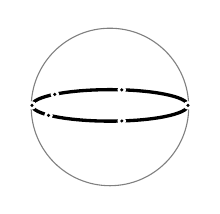
\begin{tikzpicture}[x=1cm,y=1cm]
\draw[gray,thin] (0,0) circle (1);
\draw[very thick] (0,0.02) ellipse (0.99 and 0.20);
\foreach \x/\y in {0.99/0.02,0.15/0.218,-0.7/0.16,-0.99/0.02,-0.78/-0.106,0.15/-0.178}
{\fill[white] (\x,\y) circle (0.055);\fill (\x,\y) circle (0.022);}
\end{tikzpicture}}
\margin{77}
\scanpage{79}
dont ils forment une subdivision cellulaire -- ce cercle définit une structure réelle canonique sur la droite projective complexe $\Sigma$, noté $\Sigma(\mathbb R)$, \deleted{\unsure{ou} $\Sigma_{\mathbb R}$}\inserted{$\Sigma_{\mathbb R}$}. De plus, il y a une métrique riemannienne homogène unique \inserted{(à facteur const-près)} sur $\Sigma$ invariante par $D$ (c'est pour elle que $\Sigma(\mathbb R)$ est un \uline{grand} cercle).
\margin{il est donc \deleted{\unsure{défini}}}

$\Sigma_{\mathbb R}\deleted{(\mathbb R)}$ partage $\Sigma$ en deux hémisphères, \deleted{et} en correspondance biunivoque avec $\underline\omega$ par la correspondance de Stokes
\[
(49)\qquad \pi_0(\Sigma\setminus\Sigma_{\mathbb R})\simeq\underline\omega.
\]
On a
\[
\Sigma^D=\Sigma^{D^+}=\Sigma^{\underline\omega}=\Sigma^{\{\omega\}}\unsure{\subsetneq|\subset}\Sigma\setminus\Sigma_{\mathbb R}
\qquad(\omega\in\underline\omega)
\]
et $\operatorname{card}\Sigma^D=2$, de façon précise, chacun des hémisphères ouverts contient un pt et un seul de $\Sigma^D$, d'où
\[
(50)\qquad \Sigma^D\simeq\underline\omega,
\]
on désigne par $P_\omega$ le point de $\Sigma^D$ qui correspond à $\omega\in\underline\omega$. Il est caractérisé par le fait que l'opération de $\omega$ dans l'espace tangent à $\Sigma$ en $P_\omega$ est une rotation d'angle $+2\pi/n$ (alors qu'en $P_{\omega'}$ elle est d'angle $-2\pi/n$). Pour $s\in S$, on désigne par $R_s$ le point correspondant de $\Sigma_{\mathbb R}$, pour $a\in A$ on désigne par $Q_a$ le centre de l'arête $a$.
\margin{78}
\scanpage{80}
\mspage{16}
\figure{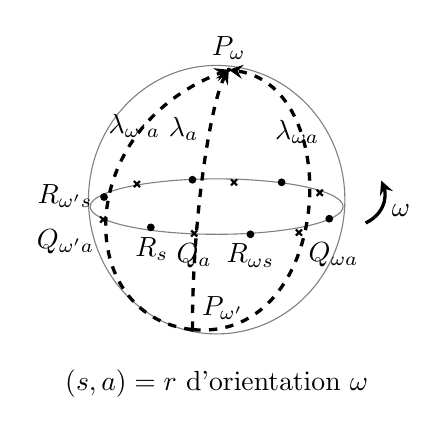
\begin{tikzpicture}[x=1.1cm,y=1.1cm,>=stealth]
\draw[gray,thin] (0,0) ellipse (1.48 and 1.55);
\draw[gray,thin] (0,-0.08) ellipse (1.46 and .32);
\coordinate (N) at (.14,1.5);\coordinate (S) at (-.28,-1.5);
\draw[very thick,dashed,->] (S) .. controls (-1.65,-1.35) and (-1.68,.8) .. (N);
\draw[very thick,dashed,->] (S) .. controls (-.28,-.1) and (-.05,1.17) .. (N);
\draw[very thick,dashed,->] (S) .. controls (1.34,-1.65) and (1.5,1.30) .. (N);
\foreach \x/\y in {-1.3/0.03,-.76/-.32,.39/-.40,1.3/-.22,.75/.20,-.28/.23}
{\fill (\x,\y) circle (.045);}
\foreach \x/\y in {-1.31/-.23,-.26/-.39,.95/-.38,1.19/.08,.20/.20,-.92/.18}
{\draw[thick] (\x-.035,\y-.035)--(\x+.035,\y+.035) (\x-.035,\y+.035)--(\x+.035,\y-.035);}
\fill (N) circle (.025);\fill (S) circle (.025);
\node[above] at (N) {$P_\omega$};\node[above right] at (S) {$P_{\omega'}$};
\node[left] at (-1.32,.04) {$R_{\omega's}$};
\node[below left] at (-1.3,-.23) {$Q_{\omega'a}$};
\node[below] at (-.75,-.32) {$R_s$};
\node[below] at (-.26,-.39) {$Q_a$};
\node[below] at (.39,-.40) {$R_{\omega s}$};
\node[below right] at (.95,-.38) {$Q_{\omega a}$};
\node at (-.95,.85) {$\lambda_{\omega'a}$};
\node at (-.38,.82) {$\lambda_a$};
\node at (.93,.78) {$\lambda_{\omega a}$};
\draw[->,very thick] (1.72,-.27) .. controls (2.00,-.13) and (1.94,.12) .. (1.90,.22);
\node[right] at (1.91,-.13) {$\omega$};
\node[below] at (0,-1.85) {$(s,a)=r$ d'orientation $\omega$};
\end{tikzpicture}}

Je m'intéresse au groupoïde fondamental
\[
\Pi_1(\underbrace{\Sigma_P\setminus S_P}_{\Sigma_P^*\text{ ou }\Sigma^*}),
\]
et je vais écrire d'abord le groupe fondamental en un $P_\omega$, correspondant au choix de $\omega\in\underline\omega$, on pose
\[
(51)\qquad
\underbrace{\Pi_{P,\omega}}_{\text{ou }\Pi_P\text{ ou }\Pi}
=\Pi_1(\Sigma_P^*,P_\omega).
\]
On considère aussi l'opération antiholomorphe unique qui fixe les pts de $\Sigma_{\mathbb R}$, et qui échange $P_\omega$ et $P_{\omega'}$, c'est la conjugaison complexe pour la structure réelle canonique de $\Sigma$, on la note $\tau$.
Ainsi, le groupe
\[
(52)\qquad D_P\times\{1,\tau\}\qquad\text{d'ordre }4n
\]
opère sur $\Sigma$, en respectant la ``carte cyclotomique'' sur $\Sigma$, le sous-groupe qui conserve l'orientation est $D_P$, celui qui induit l'identité sur $S$ (ou sur $P$) est $\{1,\tau\}$. On va aussi \uline{regarder} les groupoïdes fondamentaux mixtes de $\Sigma^*$, pour l'action sur $\Sigma^*$ de $\{1,\tau\}$, de $D_P$, ou de $D_P\times\{1,\tau\}$. \deleted{\unsure{Les groupes sont}}\inserted{On pose}
\[
(53)\qquad
\left\{
\begin{aligned}
\Pi_{P,\omega}^{\tau}&=\Pi_1(\Sigma^*,\{1,\tau\};P_\omega)\\
\Pi_{P,\omega}^{\unsure{D_*|D}}&=\Pi_1(\Sigma^*,D;P_\omega)\\
\Pi_{P,\omega}^{D,\tau}&=\Pi_1(\Sigma^*,D\times\{1,\tau\};P_\omega)
\end{aligned}
\right.
\]
en écrivant aussi $\Pi^\tau,\Pi^D,\Pi^{D,\tau}$ quand $P$ est sous-entendu.
On a donc \deleted{des} un diagramme d'inclusions de
\margin{79}
\scanpage{81}
groupes fondamentaux
\[
(54)\qquad
\diagram{\begin{tikzcd}[ampersand replacement=\&,row sep=large,column sep=large]
\&\Pi\arrow[dl,hook]\arrow[dr,hook,no head]\&\\
\Pi^D\arrow[dr,hook]\&\&\Pi^\tau\arrow[dl,hook]\\
\&\Pi^{D,\tau}\&
\end{tikzcd}}
\]
Pour exprimer commodément des générateurs remarquables de ces groupes, on introduit des chemins (indexés par \inserted{les} $a\in A$, i.e. les \uline{arêtes} du polygône)
\[
(55)\qquad \lambda_a:P_{\omega'}\longrightarrow P_\omega
\qquad
\begin{gathered}
\deleted{demi}\inserted{arc de} \text{ demi-grand cercle}\\
\text{passant par }Q_a
\end{gathered}
\]
Pour tout $s\in S$, soit
\[
\left\{
\begin{gathered}
a(s,\omega)\text{ ou }a(s)\in A\text{ tel que }(s,a)\text{ soit un repère}\\
\text{d'orientation }\omega,\text{ i.e. }
\deleted{\unsure{avec }a(\omega s,\omega)=\omega a(s,\omega)}
\inserted{s=\operatorname{or}_{\omega}(a)}
\end{gathered}
\right.
\]
\figure{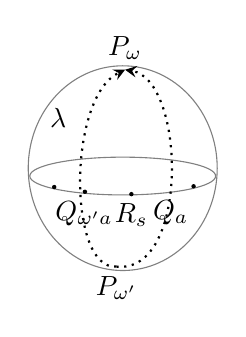
\begin{tikzpicture}[x=1cm,y=1cm,>=stealth]
\draw[gray,thin] (0,0) ellipse (1.2 and 1.3);
\draw[gray,thin] (0,-.1) ellipse (1.18 and .24);
\coordinate (N) at (.03,1.25);\coordinate (S) at (-.08,-1.25);
\draw[thick,dotted,->] (S) .. controls (-.7,-1.3) and (-.7,.9) .. (N);
\draw[thick,dotted,->] (S) .. controls (.85,-1.35) and (.8,1.12) .. (N);
\node[above] at (N) {$P_\omega$};\node[below] at (S) {$P_{\omega'}$};
\foreach \x/\y in {-.87/-.24,-.48/-.30,.11/-.33,.9/-.23}
{\fill (\x,\y) circle (.028);}
\node[below] at (-.49,-.30) {$Q_{\omega'a}$};
\node[below] at (.11,-.33) {$R_s$};
\node[below] at (.61,-.29) {$Q_a$};
\node at (-.82,.64) {$\lambda$};
\end{tikzpicture}}
on posera
\[
(56)\qquad
\begin{gathered}
\rho_s=\lambda_a\lambda_{\omega'(a)}^{-1}\\
\in\,\Pi_P=\Pi_1(\Sigma_P^*,P_\omega)
\end{gathered}
\quad
\begin{gathered}
\text{où }a=a(s,\omega),\ \omega'=\omega^{-1}\\
\text{donc }\omega'(a)=a(\omega'(s),\omega)
\end{gathered}
\]
On aura alors, pour tout $s\in S$
\[
(57)\qquad
\rho_{\omega^{n-1}s}\rho_{\omega^{n-2}s}\cdots\rho_{\omega s}\rho_s=1.
\]
Toutes ces $n$ relations sont équivalentes entre elles, si on choisit un sommet origine $s_0$ -- ce qui, avec le choix de $\omega$, fait un \uline{repère} \deleted{\unsure{de}} $r=(s_0,a(s_0,\omega))$ de $P$, d'où aussi un repère de la carte cyclotomique associée), on pose aussi
\[
(58)\qquad \rho_i=\rho_{\omega^i s_0}
\qquad
\begin{gathered}
(i\in\mathbb Z/n\mathbb Z\text{ -- les indices}\\
\text{sont notés le plus souvent}\\
0,1,\ldots,n-1
\end{gathered}
\]
de sorte que (57) prend la forme
\margin{80}
\scanpage{82}
\mspage{17}
\[
(59)\qquad \rho_{n-1}\rho_{n-2}\cdots\rho_1\rho_0=1,
\]
et on trouve en fait
\[
\textcircled{60}\qquad
\Pi_P\simeq\Pi_{P_0}\simeq
\{\rho_0,\rho_1,\ldots,\rho_{n-1}\mid
\rho_{n-1}\rho_{n-2}\cdots\rho_1\rho_0=1\},
\]
où $P_0$ désigne le polygône combinatoire-type d'ordre $n$, i.e. muni d'un épinglage par un repère.

Venons-en à $\Pi^\tau$, on introduit les
\[
(61)\qquad \tau_a=(\lambda_a,\tau)\in\Pi_P^\tau\qquad(a\in A)
\]
on trouve que
\[
\textcircled{62}\qquad \Pi^\tau\simeq\{(\tau_a)_{a\in A}\mid\tau_a^2=1\},
\]
les relations entre les $\tau_a$ et les $\rho_s$ étant données par
\[
(63)\qquad \rho_s=\tau_a\tau_{a'},\qquad
\begin{gathered}
\text{où }a,a'\text{ sont les deux arêtes incidentes}\\
\text{à }s,\ \deleted{\unsure{tel}}\text{ avec }\deleted{\unsure{que}}a=a(s,\omega)\text{ i.e.}\\
a=\omega(a')\quad\text{i.e. }a'=\omega'(a).
\end{gathered}
\]
Si on choisit \deleted{\unsure{aussi}} une arête origine $a_0$
\[
a_0=a(s_0,\omega),\quad\text{donc }(s_0,a_0)\text{ repère orienté}
\]
en écrivant
\[
(64)\qquad \tau_i=\tau_{\omega^i a_0}\qquad(i\in\mathbb Z/n\mathbb Z)
\]
on trouve donc, avec la notation (58)
\[
(65)\qquad \rho_i=\tau_i\tau_{i-1}
\]
(de sorte que la relation (59) est conséquence des relations $\tau_i^2=1$). L'écriture (62) devient
\[
(62\ \text{bis})\qquad
\Pi^\tau\simeq\{\tau_0,\ldots,\tau_{n-1}\mid
\tau_0^2=\tau_1^2\cdots=\tau_{n-1}^2=1\}.
\]
\margin{Attention, le $\tau_{a_0}$ noté ici $\tau_0$, est noté $\tau_\infty$ dans \unsure{les textes antérieurs}, pour $n=3$ (car $a_0$ est ``opposé'' au sommet $R_\infty$...).}

Considérons maintenant le stabilisateur de $P_\omega$ dans $D_P\times\{1,\tau\}$, il est formé des
\[
(66)\qquad
\widetilde g^0\unsure{:}= (g,\tau^{\alpha(g)})
\qquad
\begin{gathered}
\alpha(g)\in\mathbb Z/2\mathbb Z\\
\alpha(g)=
\begin{cases}
0&\text{si }\operatorname{sg}(g)=1\\
1&\underline{\phantom{\text{si }\operatorname{sg}(g)}}=-1
\end{cases}
\end{gathered}
\]
\margin{81}
\scanpage{83}
On a alors un hom canonique, \deleted{également} noté $g\mapsto\widetilde g$ \deleted{($\unsure{\widetilde g^0}\mapsto\widetilde g_\pi$ en cas de risque de \inserted{confusion})}
\[
(67)\qquad D\xrightarrow{\sim}(D\times\{1,\tau\})_{P_\omega}
\longrightarrow\Pi_P^{D,\tau}
\]
qui peut s'expliciter comme
\[
(68)\qquad g\mapsto\widetilde g_{\unsure{\pi}}=(1_{P_\omega},\widetilde g^0)
\]
où $1_{P_\omega}$ est le chemin \deleted{trivial} ponctuel de $P_\omega$ vers lui-même.
On trouve en particulier
\[
(69)\qquad \rho\overset{\mathrm{def}}=\widetilde\omega_\pi\in\Pi_P^D\subset\Pi_P^{D,\tau}
\qquad(\rho^n=1)
\]
et des éléments
\[
(70)\qquad \widetilde\sigma_a=(\sigma_a^0)^{\sim}_{\unsure{\pi}}\in\Pi_P^{D,\tau}
\quad\text{pour }a\in A,\quad(\widetilde\sigma_a^2=1)
\]
où
\[
(71)\qquad \sigma_a^0\in D_P
\]
est l'unique autom $\ne\mathrm{id}$ qui fixe $a$ (son action sur $\Sigma$ est la symétrie p.r. à l'axe de $\Sigma$ qui passe par $Q_a$)
\margin{Je mets l'exposant $0$, pour le distinguer de l'élément de $\Pi_P^D$ qui le représente, introduit en (72)}

On pose alors
\[
(72)\qquad \sigma_a=\widetilde\sigma_a\tau_a=\tau_a\widetilde\sigma_a
=(\lambda_a,\sigma_a^0)\in\Pi_P^D\subset\Pi_P^{D,\tau}
\]
c'est donc un élément d'\uline{ordre $2$} de $\Pi_P^D$.

\deleted{On considère les $\unsure{\rho_i}$}\inserted{Notons les formules}
\[
(73)\qquad
\left\{
\begin{aligned}
\rho(\tau_a)&=\tau_{\rho(a)}\\
\rho(\widetilde\sigma_a)&=\widetilde\sigma_{\rho(a)}\\
\rho(\sigma_a)&=\sigma_{\rho(a)}
\end{aligned}
\right.
\]
Introduisons aussi les
\[
(74)\qquad
\varepsilon_s=\sigma_{\unsure{a(s,\omega)|a}}\rho
=(\lambda_{\unsure{a}},\sigma_s^0)\in\Pi_P^D
\qquad
\begin{gathered}
s\in S\\
\text{où }a=a(s,\omega)
\end{gathered}
\]
\margin{\uline{NB} On a
$\varepsilon_s^{-1}=\rho^{-1}\sigma_a=(\lambda_{a'},\sigma_s^0)$
où $a'=\omega'a$ est l'autre arête incidente à $s$.}
\[
(75)\qquad \sigma_s^0\in D_P
\]
est l'unique autom $\ne1$ de $P$ qui fixe le sommet $s\in S$
\margin{82}
\scanpage{84}
\mspage{18}
On a alors (cf (56) pour la définition de $\rho_s$)
\[
(\unsure{76|75})\qquad
\rho_s=\varepsilon_s^2\deleted{=\rho_s}\inserted{=\sigma_a\rho\sigma_a\rho}
\quad\deleted{(\text{cf }\unsure{56})}
\]
\margin{\uline{NB}
$\rho_0=\sigma_{a_0}\rho\sigma_{a_0}\rho$
\quad
$\rho_1=\rho(\rho_0)=\rho\sigma_{a_0}\rho\sigma_{a_0}$}
Cela \inserted{((76) et (73 c))} montre que $\rho,\sigma_{a_0}$ engendrent $\Pi_P^D$, et on trouve facilement
\[
\textcircled{77}\qquad
\Pi_P^D\simeq(\rho,\sigma_{a_0}\mid\rho^n=\sigma_{a_0}^2=1)
\simeq\mathbb Z/n\mathbb Z*\mathbb Z/2\mathbb Z
\]
\margin{\uline{NB} Pour $n=3$, on identifie \unsure{dans la notation ancienne de $P$, $\infty$ au} sommet origine, et $\sigma_{a_0}$ se note alors $\sigma_\infty$.}
Car la relation (59) est déjà conséquence, moyennant (76) et (73 c), des deux relations fondamentales
\[
(78)\qquad \rho^n=1,\quad\sigma_{a_0}^2=1.
\]
Les formules (73) se complètent en
\[
(79)\qquad
\left\{
\begin{aligned}
\rho(\varepsilon_s)&=\varepsilon_{\rho(s)}\\
\rho(\rho_s)&=\rho_{\rho(s)}
\end{aligned}
\right.
\qquad(s\in S)
\]
Conséquence immédiate de (73)(74)(75), ce qui nous montre la façon dont $\rho$ opère sur $\Pi_P$.

\deleted{Quant aux $\widetilde\sigma_b$ \inserted{($b\in A$)}, ils opèrent par transport des structures
\[
(80)\qquad
\left\{
\begin{aligned}
\widetilde\sigma_b(\varepsilon_s)&=\varepsilon_{\sigma_b^0(s)}^{-1}\\
\widetilde\sigma_b(\rho_s)&=\rho_{\sigma_b^0(s)}^{-1}
\end{aligned}
\right.
\qquad\forall\,s\in S,\ b\in A
\]
Il reste à donner l'opération}
On trouve (conséquence de (65) et (62 bis))
\[
(80)\quad
\left\{
\begin{aligned}
\tau_{a_0}(\rho_0)&=\rho_0^{-1},\quad
\tau_{a_0}(\rho_1)=\rho_1^{-1},\quad
\tau_{a_0}(\rho_2)=\rho_1^{-1}(\rho_2^{-1})\\
\cdots\quad\tau_{a_0}(\rho_i)&=
(\rho_{i-1}\rho_{i-2}\cdots\rho_1)^{-1}(\rho_i^{-1})\\
&=\underbrace{(\rho_{n\deleted{\unsure{-1}}}\cdots\rho_{i+1})}_{\text{\unsure{commencer} avec }\rho_n=\rho_0,\ \uline{\text{pas}}\ \rho_{n-1}!}(\rho_i^{-1})
\end{aligned}
\right.
\quad 0\leq i\leq n-1
\]
\margin{À retenir :
$\tau_a(\rho_s)=\rho_s^{-1}$ si $s\in S$ incident à $a\in A$}
\margin{Attention, je préfère écrire $\tau_{a_0}$ au lieu de $\tau_0$, (car pour $n=3$ la ``notation reçue'' pour $\tau_{a_0}$ est $\tau_\infty$, et non $\tau_0$ !)}
\margin{\uline{NB} L'action de $\tau_a$ sur $\Pi_P$ est la composée de
\[
\tau:\Pi_1(\Sigma^*,P_\omega)\longrightarrow\Pi_1(\Sigma^*,P_{\omega'})
\]
\unsure{avec}
\[
\lambda_a:\Pi_1(\Sigma^*,P_{\omega'})\longrightarrow\Pi_1(\Sigma^*,P_\omega)
\]}
\deleted{Pour} Les relations (79) se généralisent aussitôt en
\[
\deleted{(\unsure{81|80})}\qquad
\left\{
\begin{aligned}
\widetilde g(\varepsilon_s)&=(\varepsilon_{\widetilde g^0(s)})^{\operatorname{sg}(g)}\\
\widetilde g(\rho_s)&=(\rho_{\widetilde g^0(s)})^{\operatorname{sg}(g)}
\end{aligned}
\right.
\qquad
\begin{gathered}
(g\in D_P)\\
s\in S
\end{gathered}
\]
\deleted{$\unsure{\widetilde\sigma_a}$}
\margin{\uline{NB} L'action de $\widetilde D_P\subset\Pi_P^{D,\tau}$ sur $\Pi$ est par ``transport de structures'', i.e. celle de $\widetilde D_P^0\subset D_P\times\{1,\tau\}$ sur $(\Sigma^*,P_\omega)$.}
\margin{83}
\scanpage{85}
Et en particulier, si $g$ de la forme $\sigma_a^0$, on trouve
\[
(82)\qquad
\left\{
\begin{aligned}
\widetilde\sigma_a(\varepsilon_s)&=\varepsilon_{\sigma_a^0(s)}^{-1}\\
\widetilde\sigma_a(\rho_s)&=\rho_{\sigma_a^0(s)}^{-1}
\end{aligned}
\right.
\qquad s\in S,\ a\in A
\]
\margin{donc $\widetilde\sigma_{a_0}(\rho_i)=\rho_{1-i}^{-1}$}
ce qui donne l'opération des $\widetilde\sigma_a$ sur $\Pi_P$, \deleted{\unsure{bon}} d'où \unsure{en principe} \deleted{\unsure{leur}} (avec celle des $\tau_a$) l'opération du $\Pi_P^{D,\tau}$ entier sur $\Pi_P$. \inserted{comme $\sigma_{a_0}=\widetilde\sigma_{a_0}\tau_{a_0}$} En particulier,
\[
\left\{
\begin{aligned}
\sigma_{a_0}(\rho_0)&=\rho_1,\quad
\sigma_{a_0}(\rho_1)=\rho_0,\quad
\sigma_{a_0}(\rho_i)=\tau_{a_0}(\rho_{n+1-i}^{-1})\\
&\hspace{13em}=(\rho_n\cdots\rho_{n+2-i})(\rho_{n+1-i})\\
&\hspace{13em}\text{pour }2\leq i\leq n-1.
\end{aligned}
\right.
\]
\margin{\uline{NB} L'action de $\sigma_a$ sur $\Pi_P$ est la composée de
\[
\Pi_1(\sigma_a^0):\Pi_1(\Sigma^*,P_\omega)\longrightarrow\Pi_1(\Sigma^*,P_{\omega'})
\]
avec
\[
\lambda_a:\Pi_1(\Sigma^*,P_{\omega'})\longrightarrow\Pi_1(\Sigma^*,P_\omega).
\]}

\deleted{\unsure{On}} On trouve d'ailleurs \deleted{$\Pi_P^\tau$}
\[
(\unsure{84|83})\qquad
\Pi_{P_{\unsure{c}}}^{D,\tau}\simeq\Pi_P^D\cdot\{1,\tau_{a_0}\}
\qquad\text{produit }\tfrac12\text{ direct},
\]
il faut expliciter encore l'opération de $\tau_{a_0}$ sur $\Pi_P^D$ i.e. sur $\rho$ et sur $\sigma_{a_0}$, on a
\[
(85)\qquad
\tau_{a_0}(\rho)=\sigma_{a_0}(\rho^{-1}),\quad
\tau_{a_0}(\sigma_{a_0})=\sigma_{a_0},
\]
la deuxième relation est déjà notée (72), la première s'obtient en écrivant
\[
\deleted{\rho}\tau_{a_0}
\underbrace{\rho\tau_{a_0}\rho^{-1}}_{\tau_{a_1}}
=\tau_{a_0}\tau_{a_1}
=\rho_1^{-1}
=(\rho\sigma_{a_0}\rho\sigma_{a_0})^{-1}
=\sigma_{a_0}\rho^{-1}\sigma_{a_0}\rho^{-1}
\]
d'où (85) ; \deleted{\unsure{qui s'écrit aussi}}\inserted{plus simplement} elle s'écrit
\[
\widetilde\sigma_{a_0}(\rho)=\rho^{-1}
\]
qui est triviale, puisque \deleted{pour} $\rho=\widetilde\omega$ \deleted{\unsure{de}} $g\mapsto\widetilde g$ est un hom de groupes $D_P\mathbin{-}\Pi_1^{P,\tau}$, enfin $\sigma_{a_0}^0(\rho)=\rho^{-1}\ldots$.
Il est plus joli peut-être d'écrire
\[
\textcircled{86}\quad
\left\{
\begin{aligned}
\Pi_P^{D,\tau}&\simeq\Pi_P^D\cdot\{1,\widetilde\sigma_{a_0}\}\\
\widetilde\sigma_{a_0}(\rho)&=\rho^{-1},\quad
\widetilde\sigma_{a_0}(\sigma_{a_0})=\sigma_{a_0}
\end{aligned}
\right.
\quad
\left[
\begin{gathered}
=\{\rho,\sigma_{a_0},\widetilde\sigma_{a_0}\mid
\rho^n=\sigma_{a_0}^2=\widetilde\sigma_{a_0}^{\,2}
=(\sigma_{a_0}\widetilde\sigma_{a_0})^2\\
=\widetilde\sigma_{a_0}(\rho)\rho=1\}
\end{gathered}
\right]
\]
\margin{84}
\scanpage{86}
\mspage{19}
\margin{85}
ce qui s'écrit aussi
\[
(87)\qquad
\Pi_P^{D,\tau}\simeq D(\rho)*_{D_1}D(\sigma_a)
\]
\margin{somme amalgamée de groupes sur $D_1=\{1,\widetilde\sigma_a\}$}
où
\[
(88)\qquad
\left\{
\begin{aligned}
D(\rho)&=\underbrace{D^+}_{\substack{\text{engendré}\\\text{par }\rho,\text{ avec}\\\rho^n=1}}\cdot\{1,\widetilde\sigma_a\}
\deleted{\unsure{D(\sigma_a)}}
=\text{groupe diédral d'indice }n\\
&\quad\deleted{\unsure{\simeq}}\qquad
\deleted{\unsure{défini}}\text{ par }\rho\\
D(\sigma_a)&=\{1,\sigma_a\}\times\{1,\widetilde\sigma_a\}
\quad\text{groupe diédral d'indice }2\\
&\hspace{12em}\text{défini par }\sigma_a\\
D_1&=\{1,\widetilde\sigma_a\}
\end{aligned}
\right.
\]
L'écriture (77) s'écrit aussi
\[
(89)\quad
\Pi_P^D\xrightarrow{\sim}
\Pi_{0,3}/\langle\rho_1^2,\rho_\infty^n\rangle
=\Pi_1(\mathbb P^1(\mathbb C),
\underbrace{\infty\cdot(0)+2(1)+n(\infty)}_{\text{signature}};P_+)
\]
en transformant $(\rho,\sigma_{a_0})$ en $(\rho_\infty,\rho_1)$.
Une façon a priori d'obtenir un isomorphisme (89) est de considérer la courbe complexe quotient de $\Sigma_P$ par l'action de $D_P$, \deleted{qui} action \inserted{fidèle,} qui a comme points de ramification les $R_s$ (ramification $2$), les $Q_s$ (ramification $2$), et $P_\omega,P_{\omega'}$ (ramification $n$) -- le quotient est \inserted{une courbe alg. complexe} isomorphe à $\mathbb P^1_{\mathbb C}$, l'isomorphisme étant uniquement déterminé quand on le normalise par
\[
(90)\qquad
\left\{
\begin{aligned}
R_s&\longmapsto0&&(s\in S)\\
Q_a&\longmapsto1&&(a\in A)\\
P_\omega&\longmapsto\infty&&(\omega\in\underline\omega)
\end{aligned}
\right.
\qquad(\Sigma_P\longrightarrow\mathbb P^1_{\mathbb C}).
\]
\unsure{On voit déjà} que la carte envisagée sur $\Sigma_P$ est l'image inverse de la carte universelle, par un morphisme $\Sigma_P\to\mathbb P^1_{\mathbb C}$ bien déterminé, \deleted{qui} [Dans le cas épinglé
\margin{C'est un peu une tricherie, \unsure{car} pour construire cette carte, (\unsure{chose qui n'a pas été faite}), il aurait fallu passer par ce morphisme $\Sigma_P\to\mathbb P^1_{\mathbb C}$, cf plus bas}
\scanpage{87}
\[
\tag{91}
\left\{
\begin{array}{ll}
\begin{gathered}
P=P_0=\text{polygône comb.}\\
\text{formé des }S_0=\mu_n(\mathbb C)\\
\text{et des arcs de cercle sur}\\
U=\{z\in\mathbb C\mid |z|=1\}\text{ qui}\\
\text{les joignent}
\end{gathered}
&
\begin{gathered}
\Sigma_P=\mathbb P^1_{\mathbb C}=\widehat{\mathbb C}\\
D_P^+=\mu_n(\mathbb C)\text{ opérant par homothéties}\\
\tau(z)=1/\bar z
\end{gathered}
\end{array}
\right.
\]
(cas $P$ \uline{épinglé})

\deleted{L'application}
On peut considérer que la carte envisagée \inserted{$X_n$} est l'image inverse, par
\[
z\longmapsto z^n
\qquad \mathbb P^1_{(\mathbb C)}\mathbin{-}\mathbb P^1_{(\mathbb C)}
\]
de la carte cyclotomique d'ordre $1$, $X_1$, déjà considérée (p.~7), ayant un seul sommet, un seul arc et deux faces (qui sont des monogones) (centre de l'arc $-1$, centres des faces $X_1^+$ et $X_1^-$ sont $0$ et $\infty$), qui est image inverse de la carte universelle \inserted{$X_0$:} $\{0\}\subset[0,1]\subset\mathbb P^1_{\mathbb C}$, par l'application

\figure{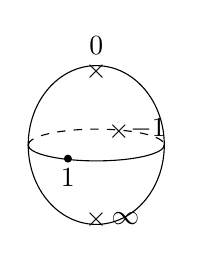
\begin{tikzpicture}[scale=.72]
\draw (0,0) ellipse (1.2 and 1.4);
\draw (-1.2,0) arc[start angle=180,end angle=360,x radius=1.2,y radius=.28];
\draw[dashed] (-1.2,0) arc[start angle=180,end angle=0,x radius=1.2,y radius=.28];
\node at (0,1.3) {$\times$}; \node[above] at (0,1.42) {$0$};
\node at (.4,.24) {$\times$};\node[right] at (.43,.28) {$-1$};
\fill (-.5,-.24) circle (2pt);\node[below] at (-.5,-.24) {$1$};
\node at (0,-1.31) {$\times$};\node[right] at (.1,-1.3) {$\infty$};
\end{tikzpicture}}

\[
z\longmapsto-\frac1{4z}(z-1)^2
\qquad \mathbb P^1(\mathbb C)\mathbin{-}\mathbb P^1(\mathbb C)
\]
(cf (23)) de sorte que l'application cherchée $X_n\longrightarrow X_0$ est
\[
\tag{92}
z\longmapsto-\frac1{4z^n}(z^n-1)^2
\]
\diagram{\begin{tikzcd}[ampersand replacement=\&]
\underbrace{X_n}_{\substack{\text{carte cycloto-}\\\text{mique type}\\\text{d'ordre }n}}
\arrow[r,"{\substack{\deleted{\unsure{g_n}}\\g_n}}"]
\&
\underbrace{X_0}_{\substack{\text{carte}\\\text{universelle}}}
\end{tikzcd}}
.\,]

Ainsi, $X_n$ devient un revêtement galoisien de $X_0$, de groupe de Galois $D_n=D_{P_0}$, ramifié comme il se doit en les seuls points $0,1,\infty$, avec en ces points la ramification $2,2,n$ respectivement, et $\Sigma_{P_0}^*=X_n^*$ devient un revêtement fini ramifié \inserted{galoisien} de $X_0\setminus\{0\}$, ramifié en les seuls points $1,\infty$, avec ramification $2,n$ en ces

\margin{86}
\scanpage{88}
\mspage{20}
points. D'après la théorie générale des groupes fondamentaux mixtes et de leurs relations avec les groupes fondamentaux à signature, on trouve donc un isomorphisme (extérieur pour le moment) canonique
\[
\tag{93}
\begin{aligned}
\Pi_1(X_n^*,\underset{\substack{\Vert\\0}}{\underline{P_{n+}}})_{\unsure{*|D}}
&\overset\sim\longrightarrow
\Pi_1(\underset{X_0\setminus\{0\}}{\underline{X_0^{\inserted{*}}}}\deleted{\unsure{,\{0\}}},2\{1\}+n\{\infty\};\underset{\exp 2i\pi/6}{\underline{P_{0+}}})\\
&\simeq\Pi_1(\underset{\mathbb P^1(\mathbb C)}{\underline{X_0}},\infty\{0\}+2\{1\}+n\{\infty\};P_{0+}).
\end{aligned}
\]
Pour trouver un isomorphisme pas extérieur, il faut changer le point base $P_{n+}=0$ en un autre, qui s'en aille dans
$\deleted{\unsure{X_0^*\setminus\{1,\infty\}}}\quad X_0^*\setminus\{1,\infty\}=X_0\setminus\{0,1,\infty\}=U_{03}$.

\figure{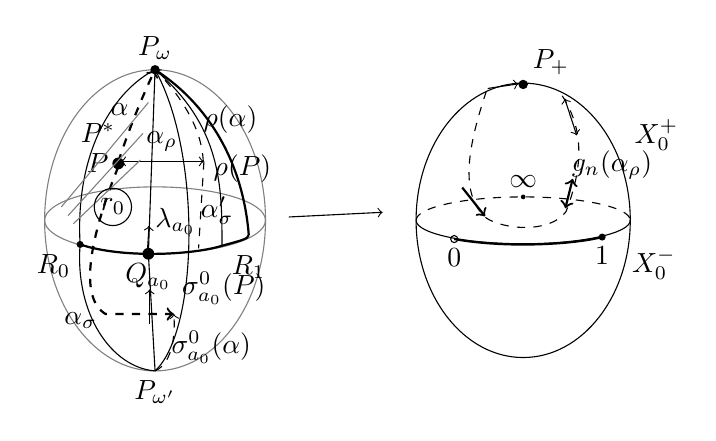
\begin{tikzpicture}[x=1cm,y=1cm,scale=.85]
\begin{scope}
\draw[gray] (0,0) ellipse (1.65 and 2.25);
\draw[gray] (-1.65,0) arc[start angle=180,end angle=360,x radius=1.65,y radius=.5];
\draw[gray] (-1.65,0) arc[start angle=180,end angle=0,x radius=1.65,y radius=.5];
\draw (-1.12,-.36) .. controls (-1.2,1.05) and (-.6,1.95) .. (0,2.25)
 .. controls (1,1.4) and (1.0,.5) .. (1,-.38);
\draw (0,2.25) .. controls (.7,1) and (.65,-1.65) .. (0,-2.25);
\draw (-1.12,-.36) .. controls (-1.2,-1.4) and (-.65,-2.2) .. (0,-2.25);
\draw[thick] (-1.12,-.36) .. controls (-.5,-.57) and (.55,-.52) .. (1,-.38)
 .. controls (1.25,-.31) and (1.4,-.28) .. (1.4,-.22);
\draw[thick] (1.4,-.22) .. controls (1.32,.8) and (.85,1.7) .. (0,2.25);
\draw (0,2.25) -- (-.1,-.5) -- (0,-2.25);
\fill (0,2.25) circle (2pt); \node[above] at (0,2.25) {$P_\omega$};
\node[below] at (0,-2.25) {$P_{\omega'}$};
\fill (-1.12,-.36) circle (1.5pt); \node[below left] at (-1.12,-.36) {$R_0$};
\fill (-.1,-.5) circle (2.5pt); \node[below] at (-.1,-.5) {$Q_{a_0}$};
\node[below right] at (1,-.38) {$R_1$};
\draw[->] (-.12,-.55) -- (-.09,-.08);
\node[right] at (-.14,-.02) {$\lambda_{a_0}$};
\fill (-.55,.85) circle (2.5pt);
\node[left] at (-.55,.85) {$P$};
\node[above left] at (-.45,1.02) {$\deleted{\unsure{P^*}}$};
\draw[dashed,->,thick] (-.55,.87) .. controls (-.38,1.4) and (-.15,1.94) .. (0,2.25);
\node[left] at (-.25,1.65) {$\alpha$};
\draw[dashed,->] (.72,.88) .. controls (.7,1.4) and (.35,1.9) .. (0,2.25);
\node[right] at (.58,1.5) {$\rho(\alpha)$};
\node[right] at (.73,.78) {$\rho(P)$};
\draw[<->] (-.51,.88) -- (.73,.88);
\node[above] at (.1,.89) {$\alpha_\rho$};
\draw[dashed] (.73,.88) -- (.65,-.42);
\node[right] at (.54,.15) {$\alpha'_\sigma$};
\draw[dashed,->,thick] (-.55,.8) .. controls (-.97,-.25) and (-1.15,-1.15) .. (-.74,-1.4) -- (.28,-1.4);
\node[left] at (-.72,-1.5) {$\alpha_\sigma$};
\node[above right] at (.26,-1.4) {$\sigma^0_{a_0}(P)$};
\draw[dashed,->] (0,-2.25) .. controls (.28,-2.13) and (.3,-1.65) .. (.28,-1.4);
\node[right] at (.1,-1.9) {$\sigma^0_{a_0}(\alpha)$};
\draw[->] (-.08,-1.55) -- (-.08,-1.03);
\draw[gray] (-1.4,.2) -- (-.1,1.76);
\draw[gray] (-1.3,.07) -- (-.18,1.3);
\draw[gray] (-1.22,-.05) -- (-.22,.9);
\node[draw,circle,inner sep=1pt] at (-.63,.2) {$r_0$};
\end{scope}
\draw[->] (2,.05) -- (3.4,.12);
\begin{scope}[shift={(5.5,0)}]
\draw (0,0) ellipse (1.6 and 2.05);
\draw (-1.6,0) arc[start angle=180,end angle=360,x radius=1.6,y radius=.35];
\draw[dashed] (-1.6,0) arc[start angle=180,end angle=0,x radius=1.6,y radius=.35];
\draw[thick] (-1.03,-.28) .. controls (-.25,-.42) and (.75,-.36) .. (1.18,-.25);
\draw (-1.03,-.28) circle (1.5pt); \node[below] at (-1.03,-.28) {$0$};
\fill (1.18,-.25) circle (1.5pt); \node[below] at (1.18,-.25) {$1$};
\fill (0,.35) circle (1pt); \node[above] at (0,.35) {$\infty$};
\fill (0,2.03) circle (2pt); \node[above right] at (0,2.03) {$P_+$};
\node[right] at (1.52,1.27) {$X_0^+$};
\node[right] at (1.48,-.65) {$X_0^-$};
\draw[->] (-.53,1.97) -- (-.07,2.04);
\draw[dashed] (-.55,1.93) .. controls (-.82,1.12) and (-.96,.4) .. (-.56,.04)
 .. controls (-.3,-.14) and (.4,-.2) .. (.64,.13)
 .. controls (.88,.76) and (.94,1.35) .. (.55,1.91);
\draw[->,thick] (-.91,.49) -- (-.57,.06);
\draw[<->,thick] (.63,.18) -- (.74,.62);
\draw[<->] (.8,1.27) -- (.62,1.82);
\node[right] at (.58,.83) {$g_n(\alpha_\rho)$};
\end{scope}
\end{tikzpicture}}

On considère la subdivision barycentrique de la carte $X_n$, image inverse de la subdivision barycentrique de $X_0$, dont les deux faces sont les deux hémisphères $X_0^+$ et $X_0^-$ — les images inverses de celles-ci sont les $4n$ ``repères'' \inserted{ou ``drapeaux''} de la subdivision barycentrique de $X_n$, \deleted{qui} \inserted{dont les $2n$ repères \uline{directs}} correspondent aux $2n$ repères du polygone $P$. L'épinglage de ce dernier nous fournit un repère origine
\[
\tag{94} r_0=(R_0,Q_{a_0},P_\omega)\qquad
(\mathrel{\overset\sim\longmapsto}X_0^+)
\]
qui par $g_n$ est appliqué homéomorphiquement sur $X_0^+$, avec \deleted{$R_0\longmapsto$}
\[
g_n:\quad R_0\longmapsto0,\quad Q_{a_0}\longmapsto1,\quad P_\omega\longmapsto\infty
\]
Prenant le point $P\in r_0$ qui s'envoit sur le ``pôle nord'' $P_+$ $(=\exp 2i\pi/6)\in X_n^+$,
\[
g_n:\qquad P\longmapsto P_+.
\]

\margin{87}
\scanpage{89}
La théorie générale donne un iso (pas extérieur !)
\[
\tag{95}
\begin{aligned}
\Pi_1(X_n^*,\inserted{D_n;}P)
&\overset\sim\longrightarrow
\Pi_1(\underset{\overset{\mathrm{def}}=X_0\setminus\{0\}}{\underline{X_0^{\unsure{*|**}}}},2\{1\}+n\{\infty\};P_+)\\
&\simeq\Pi_{0,3}/\langle\rho_1^2,\rho_\infty^n\rangle,
\end{aligned}
\]
pour obtenir un isomorphisme précisé (93), il faut composer (95) avec un isomorphisme
\[
\tag{96}
\Pi_1(X_n^*,\inserted{D_n;}P_+)\overset\sim\longrightarrow
\Pi_1(X_n^*,D_n,P)
\]
déduit d'une classe de chemins $P_+\mathbin{-}P$ dans $X_n^*$ — on prendra la \inserted{l'unique} classe de chemins provenant d'un chemin $\alpha$ \uline{dans $r_0$}, comme choix le plus naturel, ce qui précise 96. L'homomorphisme (95), quant à lui, est donné par la formule des plus évidentes
\[
(l,g)\longmapsto g_n(l)
\]
où $g\in D_n$, $\underbrace{l:g(P_{\unsure{*|+}})\longrightarrow P_{\unsure{*|+}}}_{\substack{\text{chemin dans}\\X_n^*,\text{ ou mieux,}\\\text{chemin dans }X_n^{\unsure{***|**}}\\
=X_n^*\setminus\{(Q_a),P_\omega,P_{\omega'}\}\\
=X_n\setminus\{\text{pts de ramification}\}\\
=X_n\mid U_{03}}}$,
d'où $g_n(l):g_n(P)\longrightarrow g_n(P)$ un lacet en $P_+=g_n(P)$ dont on prend la classe dans le quotient de $\Pi_{03}$ — qui ne dépend pas du choix fait, mais seulement de l'élément de $\Pi_1(X_n^*,D_n;P)$ représenté par $(l,g)$ --.

Considérons donc l'application composée de (95)(96), qui \deleted{\unsure{$g_n$}} \inserted{non extérieure canonique}
\[
\tag{97}
\begin{aligned}
\Pi_1(X_n^*,D_n;P_+)&\xrightarrow{\deleted{\unsure{g}}\ g_n}
\Pi_1(X_0,\infty\{0\}+2.\{1\}+n\{\infty\};P_+)\\
&\simeq\Pi_{03}/\langle\rho_1^2,\rho_\infty^n\rangle
\end{aligned}
\]
et calculons ses valeurs pour $\rho,\sigma_{a_0}$. L'image de $\rho$ par 96, est donné par le chemin
\[
\rho(P)\xrightarrow{\alpha_\rho}\deleted{\unsure{P_+}}P^{\unsure{*|+}}
\quad\text{dans }X_n^{\unsure{***|**}}
\]
que fournit le 1-squelette de la subdivision

\margin{NB $\alpha_\rho$ est obtenu par déformation dans $X_n^{\unsure{*|**}}$ du chemin composé $\alpha\circ\rho(\alpha)^{-1}$.}

\margin{88}
\scanpage{90}
\mspage{21}
barycentrique juste deux fois, \deleted{\unsure{en}} en traversant respectivement les côtés $P_\omega R_1$ $(\overset{g_n}\longmapsto(\widehat{\infty,0}))$ et $P_\omega Q_{a_0}$ $(\overset{g_n}\longmapsto(\infty,1))$ — donc $g_n(\alpha_\rho)$ est un lacet dans $U_{0,3}=X_0^*\setminus\{1,\infty\}$ \deleted{qui} en $P_+$, qui \deleted{franchit} traverse une fois l'arc $\widehat{(\infty,0)}$ de l'équateur, une fois l'arc $\widehat{(\infty,1)}$, dans cet ordre. Sa classe dans $\Pi_{0,3}$ est donc $\rho_\infty^{-1}$:
\[
\tag{*} g_n(\rho)=\rho_\infty^{-1}.
\]
\deleted{L'élément de} \inserted{L'image de} $\sigma_{a_0}=(\lambda_{a_0},\sigma^0_{a_0})$ par (96) est représentée par $\sigma^0_{a_0}(P)\longrightarrow P$, qui est le composé dans $\Pi_1(X_n^*)$ \deleted{du \unsure{chemin}} $\alpha\lambda_{a_0}\sigma^0_{a_0}(\alpha)^{-1}$, lequel chemin peut se déformer en le chemin \deleted{$\unsure{\alpha_{a_0}}$}
\[
\alpha_{\sigma\deleted{\unsure{a_0}}}:\sigma^0_{a_0}(P)\longrightarrow P
\]
situé tout entier dans $X_n^{\unsure{***|**}}$, qui franchit le 1-squelette \inserted{de la} subdivision barycentrique en exactement deux pts, qui sont respectivement sur les arcs $P_\omega,Q_{a_0}$ $(\overset{g_n}\longmapsto\widehat{(\infty,1)})$ et $(Q_{a_0},R_0)$ $(\overset{g_n}\longmapsto\widehat{(0,1)})$, donc $g_n(\alpha_\sigma)$ est un lacet en $P_+$ qui franchit $\widehat{(\infty,1)}$ puis $\widehat{(0,1)}$ dans cet ordre, donc qui \deleted{est} a la classe $\rho_1^{-1}$. On aurait pu prendre aussi $\alpha'_\sigma:\sigma^0_{a_0}(P)\mathbin{-}P$, franchissant d'abord $(Q_{a_0},R_1)$ $(\overset{g_n}\longmapsto\widehat{(0,1)})$ puis $(Q_{a_0},P_\omega)$ $(\overset{g_n}\longmapsto(1,\infty))$ — \deleted{aurait} trouverait $g_n(\alpha'_\sigma)=\rho_1$ — mais dans le quotient $\Pi_{03}/\langle\rho_1^2,\rho_{\unsure{\infty|0}}^n\rangle$, $\rho_1$ et $\rho_1^{-1}$ ont $\unsure{=|\overline m}$ image, comme il se doit. Donc on trouve
\[
\tag{bis} g_n(\sigma_{a_0})=\rho_1\quad(=\rho_1^{-1})
\]

\margin{89}
\scanpage{91}
et en composant (*) et (**) on trouve
\[
g_n(\underset{\sigma_{a_0}\rho}{\underline{\varepsilon_0}})
=g_n(\sigma_{a_0})g_n(\rho)
=\rho_1^{-1}\rho_\infty^{-1}
=(\rho_\infty\rho_1)^{-1}=\rho_0
\]
En résumé, on trouve donc
\[
\tag{98}
\left\{
\begin{gathered}
g_n:\Pi_1(X_n^*,D_n;P_{n+})\overset\sim\longrightarrow
\Pi_{0,3}/\langle\rho_1^2,\rho_\infty^n\rangle
=\Pi_1(\underset{\mathbb P^1_{\mathbb C}}{\underline{X_0}},
\underbrace{\infty\{0\}+2\{1\}+n\{\infty\}}_{\text{signature }\vec\nu_n};P_+)\\
\varepsilon_0\longmapsto\rho_0\\
\sigma_{a_0}\longmapsto\rho_1=\rho_1^{-1}\\
\rho\longmapsto\rho_\infty^{-1}
\end{gathered}
\right.
\]
Par le même principe, on trouve un isomorphisme
\[
\tag{99}
\begin{aligned}
g_n:\Pi_1(X_n^*,D_n\times\{1,\tau\};P_{n+})
&\overset\sim\longrightarrow\Pi_1(X_0,\underline{\vec\nu_n},\{1,\tau\};P_+)\\
\simeq\Pi_{\unsure{n|P}}^{D,\tau}\simeq\Pi_n^D.\{1,\widetilde\sigma_{a_0}\}
&\simeq(\Pi_{0,3}/\langle\rho_1^2,\rho_\infty^n\rangle).\{1,\widetilde\tau_\infty\}
\end{aligned}
\]

\margin{\uline{NB}
$\tau_\infty(\rho_0)=\rho_0^{-1}$\\
$\tau_\infty(\rho_1)=\rho_1^{-1}$\\
$\tau_\infty(\rho_\infty)=\rho_0(\rho_\infty^{-1})$\\
cf (80) dans le cas $n=3$, ici $\tau_\infty=\tau_{a_0}$ par définition \ldots}

qui prolonge $(97)=(98)$, et qui se calcule de la $\unsure{=|\overline m}$ façon. Il suffit, pour achever de déterminer $g_n$, de calculer sa valeur sur \deleted{$\unsure{\sigma_{a_0}}$}
$\widetilde\sigma_{a_0}=(1_{P_+},\widetilde\sigma^0_{a_0})$.
Ici $\widetilde\sigma^0_{a_0}$ agit sur $X_n$ par la symétrie par un grand cercle $P_\omega Q_{a_0}P_{\omega'}$, \deleted{\unsure{son}} son image dans
$\Pi_1(X_n^*,D_n\times\{1,\tau\};P)$ est défini par le chemin \deleted{$\unsure{P}$}
\[
P'=\widetilde\sigma^0_{a_0}(P)\longrightarrow P
\]
donné par $\alpha\circ\alpha'^{-1}$, où $\alpha'=\widetilde\sigma^0_{a_0}(\alpha)$, ce chemin est homotope dans $X_n^{\unsure{2|*}}$ au chemin $\widetilde\alpha_\sigma$, \deleted{qui} dans $X_n^{\unsure{***|**}}$, qui franchit la subdivision barycentrique une seule fois, en $P_+Q_{a_0}$ $(\overset{g_n}\longmapsto(\infty,1))$.

\figure{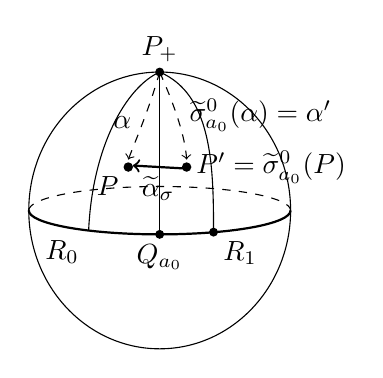
\begin{tikzpicture}[scale=.95]
\draw (0,0) ellipse (1.75 and 1.85);
\draw[thick] (-1.75,0) arc[start angle=180,end angle=360,x radius=1.75,y radius=.32];
\draw[dashed] (-1.75,0) arc[start angle=180,end angle=0,x radius=1.75,y radius=.32];
\draw (-.95,-.27) .. controls (-.9,.85) and (-.45,1.65) .. (0,1.85)
 .. controls (.7,1.55) and (.72,.6) .. (.72,-.29);
\draw (0,1.85) -- (0,-.32);
\fill (0,1.85) circle (1.7pt); \node[above] at (0,1.85) {$P_+$};
\node[below left] at (-.95,-.27) {$R_0$};
\fill (0,-.32) circle (1.7pt); \node[below] at (0,-.32) {$Q_{a_0}$};
\fill (.72,-.29) circle (1.7pt); \node[below right] at (.72,-.29) {$R_1$};
\fill (-.42,.58) circle (1.8pt); \node[below left] at (-.42,.58) {$P$};
\fill (.36,.58) circle (1.8pt); \node[right] at (.36,.58) {$P'=\widetilde\sigma^0_{a_0}(P)$};
\draw[dashed,->] (0,1.85) .. controls (-.14,1.36) and (-.3,.99) .. (-.42,.68);
\node[left] at (-.25,1.17) {$\alpha$};
\draw[dashed,->] (0,1.85) .. controls (.2,1.4) and (.34,.99) .. (.36,.68);
\node[right] at (.27,1.27) {$\widetilde\sigma^0_{a_0}(\alpha)=\alpha'$};
\draw[thick,->] (.35,.56) -- (-.36,.6);
\node[below] at (-.02,.58) {$\widetilde\alpha_\sigma$};
\end{tikzpicture}}

\margin{90}
\scanpage{92}
\mspage{22}
Par $g_n$ ce chemin devient un chemin dans $U_{03}$
\[
g_n(\widetilde\alpha_\sigma):
g_n(P')=g_n(\widetilde\sigma^0_{a_0}(P))=\tau g_n(P)=\tau(P_+)=P_-
\longrightarrow g_n(P)=P_+
\]
qui franchit l'équateur \deleted{\unsure{sur l'arc}} exactement une fois, en traversant l'arc $\widehat{(1,\infty)}$ — c'est donc $\tau_{a_1}$, noté aussi $\tau_0$ (car $a_1$ est opposé au sommet $0$) donc on trouve

\figure{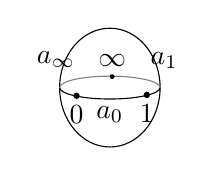
\begin{tikzpicture}[scale=.58]
\draw (0,0) ellipse (1.1 and 1.3);
\draw (-1.1,0) arc[start angle=180,end angle=360,x radius=1.1,y radius=.25];
\draw[gray] (-1.1,0) arc[start angle=180,end angle=0,x radius=1.1,y radius=.25];
\fill (-.73,-.18) circle (2pt); \node[below] at (-.73,-.18) {$0$};
\fill (.81,-.16) circle (2pt); \node[below] at (.81,-.16) {$1$};
\fill (.05,.24) circle (1.5pt); \node[above] at (.05,.24) {$\infty$};
\node[below] at (0,-.2) {$a_0$};
\node[above left] at (-.55,.22) {$a_\infty$};
\node[above right] at (.68,.2) {$a_1$};
\end{tikzpicture}}

\deleted{(99)}
\[
\tag{*} g_n(\widetilde\sigma_{a_0})=\tau_0\in
\Pi_{0,3}^{\tau}/\langle\rho_1^2,\rho_\infty^n\rangle
\]
\deleted{$\unsure{a}$}
pour se rassurer on vérifiera que conformément à (86), $\widetilde\sigma_{a_0}(\rho)=\rho^{-1}$, $\widetilde\sigma_{a_0}(\sigma_{a_0})=\sigma_{a_0}$, on a bien
\[
\tau_0(\rho_\infty^{-1})=\rho_\infty^{\deleted{\unsure{-1}}},\quad
\tau_0(\rho_1)=\rho_1^{-1}
\]
ce qui est contenu en effet dans les (deux premières) formules (80) pour $n=3$, en prenant ici pour $a_0$ le côté $(1,\infty)$ du triangle $(0,1,\infty)$ \deleted{\unsure{dans}} dans $X_0$ \ldots. On tire de \deleted{(99)} (*)
\[
g_n(\tau_{a_0})=g_n(\widetilde\sigma_{a_0}.\sigma_{a_0})
=g_n(\widetilde\sigma_{a_0})g_n(\sigma_{a_0})
=\tau_0\rho_1=\tau_\infty
\]
puisque $\rho_1=\tau_0\tau_\infty$, \deleted{donc} en résumé
\[
\tag{100}
g_n(\widetilde\sigma_{a_0})=\tau_0,\quad g_n(\tau_{a_0})=\tau_\infty.
\]

\figure{\begin{tikzpicture}\draw (0,.6)--(.55,0);\end{tikzpicture}}

7: Dans toutes ces considérations, \inserted{du § 6} on a un peu perdu de vue les cartes, dont il n'a plus été question. Pourtant, le groupe $\Pi_P^\tau$ s'interprète comme le groupe ``cartographique pondéré $\unsure{n}$-polygonal'', qui est tel que

\margin{91}
\scanpage{93}
\mspage{\unsure{R|B}}
les \deleted{\unsure{en}} ensembles finis à opér. $\Pi_P^\tau$ — i.e. munis d'endomorphismes \deleted{$\tau_a\ (a\in A)$} involutifs $\tau_a$, indexés par les \uline{côtés} de $P$ — s'interprètent en termes de telles cartes, mais en supposant que les $\tau_a$ opèrent sans points fixes. \deleted{Pour \unsure{cela}}

\margin{Une pondération du type $P$}

Si on associe à la carte $X$ $P$-pondérée l'ensemble \inserted{$R(X)$} de ses \uline{faces}, on trouve en effet un ensemble avec des opérations $\tau_a$, \inserted{où $\tau_a$} correspondant \deleted{\unsure{une}} \inserted{à la} symétrie par r. \deleted{aux} à l'arête de type $a$ d'une face. Ici, la pondération (disons, numérotation circulaire) des \deleted{\uline{faces}} \inserted{\uline{arêtes} d'une \uline{face}} apparaît plus commode que celle des sommets. Le foncteur

\figure{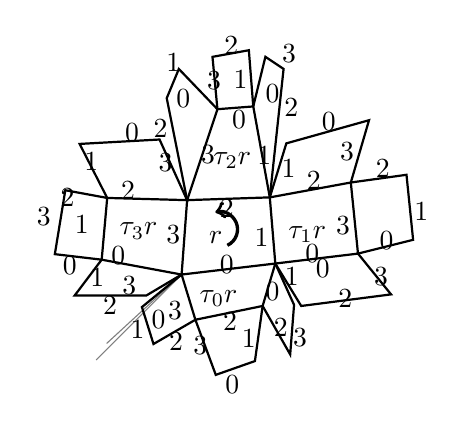
\begin{tikzpicture}[scale=.7]
\coordinate (A) at (0,0); \coordinate (B) at (1.5,.05);
\coordinate (C) at (1.6,-1.15); \coordinate (D) at (-.1,-1.35);
\draw[gray,thin] (D)--(-1.65,-2.9);
\draw[gray,thin] (D)--(-1.46,-2.6);
\draw[thick] (A)--(B)--(C)--(D)--cycle;
\draw[thick] (A)--(.55,1.65)--(1.2,1.7)--(B);
\draw[thick] (.55,1.65)--(.46,2.6)--(1.12,2.72)--(1.2,1.7);
\draw[thick] (A)--(-.37,1.85)--(-.15,2.38)--(.55,1.65);
\draw[thick] (B)--(1.75,2.38)--(1.42,2.6)--(1.2,1.7);
\draw[thick] (A)--(-1.45,.04)--(-1.95,1.02)--(-.5,1.1)--cycle;
\draw[thick] (-1.45,.04)--(-1.55,-1.08)--(D);
\draw[thick] (-1.45,.04)--(-2.21,.18)--(-2.4,-.98)--(-1.55,-1.08);
\draw[thick] (-1.55,-1.08)--(-2.04,-1.73)--(-.74,-1.73)--(D);
\draw[thick] (D)--(.15,-2.17)--(1.37,-1.92)--(C);
\draw[thick] (.15,-2.17)--(.52,-3.17)--(1.23,-2.92)--(1.37,-1.92);
\draw[thick] (D)--(-.82,-1.94)--(-.61,-2.61)--(.15,-2.17);
\draw[thick] (C)--(1.94,-1.9)--(1.87,-2.8)--(1.37,-1.92);
\draw[thick] (B)--(2.97,.32)--(3.1,-.97)--(C);
\draw[thick] (B)--(1.8,1.03)--(3.3,1.45)--(2.97,.32);
\draw[thick] (2.97,.32)--(3.98,.46)--(4.1,-.72)--(3.1,-.97);
\draw[thick] (C)--(2.07,-1.92)--(3.7,-1.71)--(3.1,-.97);
\node at (.52,-.68) {$r$};
\draw[very thick,->] (.73,-.82) arc[start angle=-65,end angle=105,radius=.32];
\node at (.82,.72) {$\tau_2r$};
\node at (-.88,-.56) {$\tau_3r$};
\node at (2.18,-.62) {$\tau_1r$};
\node at (.57,-1.78) {$\tau_0r$};
\foreach \x/\y/\z in {
.72/-.15/2,1.35/-.68/1,.72/-1.17/0,-.25/-.63/3,
.94/1.47/0,.38/.82/3,1.4/.81/1,
.49/2.17/3,.97/2.18/1,.8/2.8/2,
-.07/1.85/0,-.48/1.3/2,-.25/2.5/1,
1.55/1.94/0,1.89/1.68/2,1.85/2.66/3,
-1.07/.17/2,-1/1.23/0,-1.74/.7/1,-.39/.68/3,
-1.25/-1/0,-1.91/-.45/1,-2.17/.05/2,-2.6/-.3/3,-2.13/-1.18/0,
-1.63/-1.41/1,-1.05/-1.55/3,-1.4/-1.91/2,
-.52/-2.16/0,-.22/-2/3,-.9/-2.35/1,-.2/-2.57/2,
.78/-2.2/2,1.12/-2.52/1,.24/-2.63/3,.82/-3.35/0,
1.55/-1.65/0,1.7/-2.32/2,2.05/-2.5/3,1.9/-1.38/1,
2.27/-.97/0,2.83/-.47/3,
1.84/.58/1,2.3/.35/2,2.9/.89/3,2.57/1.43/0,
3.55/.57/2,4.25/-.2/1,3.62/-.73/0,
2.46/-1.24/0,2.87/-1.79/2,3.52/-1.38/3}
{\node at (\x,\y) {$\z$};}
\end{tikzpicture}}

\diagram{\begin{tikzcd}[ampersand replacement=\&,column sep=large]
X\arrow[r,mapsto]\&R(X)\\
\begin{gathered}\text{cartes $P$-pondérées}\\\text{finies}\\(\text{cat. isotopique})\end{gathered}
\arrow[r,"\approx"]\&
\begin{gathered}\Pi_P^\tau\text{-ensembles finis}\\\text{spéciaux}\\
(\text{i.e. où les }\tau_i\\\text{opèrent ss pt fixe})\end{gathered}
\end{tikzcd}}
(\unsure{100|101})

est une équivalence des catégories. \deleted{L'équivalence} \inserted{Elle induit une équivalence}
\deleted{qui \unsure{à un} \unsure{$N$} \unsure{vient} \unsure{on associe à} $N$}
\deleted{$\Pi_P^\tau$-\unsure{ensembles}}

\diagram{\begin{tikzcd}[ampersand replacement=\&,column sep=large]
\begin{gathered}\text{cartes $P$-pondérées }\deleted{\text{étales}}\\\text{finies \uline{orientées}}\end{gathered}
\arrow[r,"\approx"]\&
\Pi_P\text{-ens. finis}\\
\&X\arrow[r,mapsto]\&R^+(X)
\end{tikzcd}}
(102)

en associant à chaque telle carte l'ens $R^+(X)$ de ses \deleted{repères} faces ``directes'', i.e. \deleted{que} dont l'orientation induite par $X$ est celle définie par $\omega\in\underline\omega$, définissant un ordre circulaire sur l'ens des sommets (ou des arêtes)

\margin{92}
\scanpage{94}
\mspage{23}
de la face. On notera que pour décrire le groupe $\Pi_P^\tau$, et l'équivalence (101), on n'a pas besoin d'autre donnée que du pol. combinatoire $P$, le groupe $\Pi_P^\tau$ est défini simplement par (62) (sans référence au choix d'un point-base $P_\omega$ dans un espace $\Sigma_P^*$ !). Par contre, pour définir $\Pi_P$ et l'équivalence (102), on a besoin du choix d'une orientation $\omega$ de $P$, ce qui permet d'introduire $\Pi_P$ p. ex. comme $\Pi_1(\Sigma_P^*,P_\omega)$. À vrai dire, on pourrait définir $\Pi_P$, sans choix de $\omega$, comme noyau de l'hom. can. $\Pi_P^\tau\unsure{\mathbin{-}|\longrightarrow}\{\pm1\}$, de façon à avoir la suite exacte

\diagram{\begin{tikzcd}[ampersand replacement=\&]
1\arrow[r]\&\Pi_P\arrow[r,no head]\&\Pi_P^\tau\arrow[r]\&\{\pm1\}\arrow[r,no head]\&1\\
\&\&\tau_a\arrow[r,mapsto]\&-1
\end{tikzcd}}
(103)

mais il reste que le choix d'un foncteur (102) dépend du choix d'une orientation $\omega$ de $P$.

Un foncteur quasi-inverse de (102) s'obtient en interprétant le deuxième \unsure{mb} par la théorie de Galois des revêtements étales de $\Sigma_P^*$

\diagram{\begin{tikzcd}[ampersand replacement=\&,column sep=large]
\Pi_P\text{-ens finis}\arrow[r,"\approx"]\&
\begin{gathered}\text{revêtements ramifiés}\\
\text{finis de }\Sigma_P,\text{ étales}\\
\text{au dessus de }\Sigma_P^*
\end{gathered}
\end{tikzcd}}
(104)

si on a un tel rev. \deleted{étale} $X$ de $\Sigma_P$, l'image inverse de la carte \deleted{\unsure{qui est}} \inserted{canonique} sur $\Sigma_P$ (\unsure{jouant} le rôle de \uline{carte, $P$-pondérée orientée universelle})

\margin{93}
\scanpage{95}
\deleted{\mspage{\unsure{24}}}
est la carte $P$-pondérée \inserted{orientée} cherchée.

Pour avoir un foncteur quasi inverse de (101), on procède de façon analogue, en utilisant une orientation de $P$. (Sinon, on utilise l'ens $\underline\omega$ pour tordre le corps $\mathbb C$, et le remplacer par $\mathbb C(\omega)$, et on considère \deleted{la sphère} $\mathbb C(\omega)$-variété $\Sigma_P(\mathbb C(\omega))$ au lieu de $\Sigma_P(\mathbb C)$, qui aura un point canonique $P_+$ pouvant servir de pt base). On \deleted{passe} interprète $\Pi_P^\tau$ comme $\Pi_1(\Sigma_P^*,\{1,\tau\};P_\omega)$, et on procède comme p.~9 (dans le cas $n=3$, dont on a ici une généralisation \ldots).

Sûrement on doit pouvoir généraliser aussi au cas quelconque, les considérations du § 5 (p.~$12'$--14), qui précisent (en relation avec \deleted{\unsure{les}} les iso. (97) (99)) les relations entre cartes $P$-pondérées, et cartes $n$-gonales (i.e. dont toutes les faces sont $n$-gonales \ldots). Je ne vais pas détailler ce point ici.

\margin{94}
\scanpage{96}
\mspage{24}
8. Une façon d'obtenir une configuration ``polygône régulier à $n$ côtés'' \inserted{$P_n$} dans une sphère complexe \inserted{$\Sigma$}, \deleted{est} i.e. dans une droite projective complexe, est de partir d'un polygone régulier à $2n$ côtés $\widetilde P_{2n}$ (\unsure{moralement}, un revêtement de degré $2$ de $P_n$), plongé dans un \deleted{espace} \inserted{plan} vectoriel réel $V_{\widetilde P_{2n}}$ (en tant que polygône régulier) et de poser

\margin{$P_n=P=(S,A,R\subset S\times A)$}

\[
\tag{1}\Sigma=\mathbb P(V_{\widetilde P_{2n}})(\mathbb C)
\]
en prenant
\[
\tag{2}P_n=\widetilde P_{2n}/\{\pm1\}
\]
\margin{\uline{NB} $-1$ opère sur le polygone combinatoire $P_{2n}$ par antipodisme}

\deleted{et en} donc
\[
S=\widetilde S/\pm1,\quad A=\widetilde A/\pm1,\quad R=\widetilde R/\pm1,
\]
et en définissant le plongement
\[
\tag{3}S\hookrightarrow\Sigma
\]
par passage au quotient en termes de
(
\diagram{\begin{tikzcd}[ampersand replacement=\&]
\widetilde S\arrow[r]\&\Sigma\\
R_{\tilde s}\arrow[r,mapsto]\&
\mathbb C.R_{\tilde s}\in\mathbb P(V_{\mathbb C})\unsure{\{=|(=}\mathbb P(V)(\mathbb C).
\end{tikzcd}}

\deleted{De cette} En fait, \deleted{L'application (3) se \unsure{factorise}} \inserted{par construction $\Sigma$ provient} de la droite projective \uline{réelle} $\mathbb P(\underset{V}{\underline{V_{\widetilde P_{2n}}}})$, et l'application (3) se factorise par \deleted{$\Sigma_{\mathbb R}\Vert$}
\[
\tag{4}\Sigma_{\mathbb R}=\boldsymbol\Sigma_{\widetilde P_{2n}}(\mathbb R)
\]
où on a posé
\[
\tag{5}
\underset{\substack{\Vert\\\boldsymbol\Sigma_{P_n}}}{\boldsymbol\Sigma_{\widetilde P_{2n}}}
=\mathbb P(V_{\widetilde P_{2n}})
\quad\text{(ne dépend en fait que de }P_n=\widetilde P_{2n}/\pm1\text{)}
\]

\margin{95}
\scanpage{97}
La représentation naturelle de \deleted{$D_{\widetilde P}$}
\[
\tag{6}D_{\widetilde P_{2n}}\overset{\mathrm{def}}=\operatorname{Aut}_{\mathrm{comb}}(\widetilde P_{2n})
\qquad(\simeq D_{2n})
\]
sur $V_{\widetilde P_{2n}}$ définit une action de $D_{\widetilde P_{2n}}$ sur $\boldsymbol\Sigma_{\widetilde P_{2n}}$ et par là sur $\Sigma$, mais qui est triviale sur le sous-groupe $\pm1$, et se factorise donc par une action de
\[
\tag{7}D_{P_n}\overset{\mathrm{def}}=\operatorname{Aut}_{\mathrm{comb}}(P_n)
\simeq D_{\widetilde P_{2n}}/\{\pm1\}
\]
sur $\Sigma=\Sigma_{P_n}$, qui n'est autre que son action naturelle par transport des structures, quand on interprète $\Sigma$ directement comme défini en termes de $P_n$.

\deleted{\unsure{Si}} Si $n$ est impair, la suite exacte canonique

\diagram{\begin{tikzcd}[ampersand replacement=\&]
1\arrow[r,no head]\&\{\pm1\}\arrow[r,no head]\&D_{\widetilde P_{2n}}\arrow[r,no head]\&D_{P_n}\arrow[r,no head]\&1
\end{tikzcd}}
(8)

est scindée \deleted{naturellement} (le \inserted{choix d'un} scindage dépendant du choix d'un \inserted{des deux} ``sous-$n$-gônes'' $P'_n,P''_n$ du $2n$-gône combinatoire $\widetilde P_{2n}$ (pour $n=6$, le choix d'un des deux triangles $ABC$, $A'B'C'$ marqués sur la figure). Cela est lié au fait qu'on a une équivalence de catégories, \uuline{pour $n$ impair}

\figure{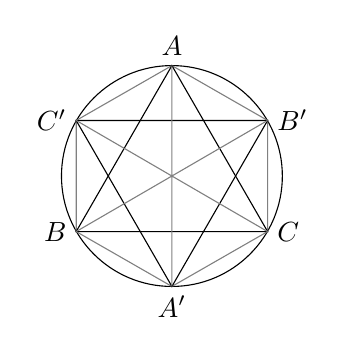
\begin{tikzpicture}[scale=.85]
\coordinate (A) at (0,1.65);
\coordinate (Bp) at (1.43,.83);
\coordinate (C) at (1.43,-.83);
\coordinate (Ap) at (0,-1.65);
\coordinate (B) at (-1.43,-.83);
\coordinate (Cp) at (-1.43,.83);
\draw (0,0) circle (1.65);
\draw[gray] (A)--(Bp)--(C)--(Ap)--(B)--(Cp)--cycle;
\draw (A)--(B)--(C)--cycle;
\draw (Ap)--(Bp)--(Cp)--cycle;
\draw[gray] (A)--(Ap) (B)--(Bp) (C)--(Cp);
\node[above] at (A) {$A$};
\node[right] at (Bp) {$B'$};
\node[right] at (C) {$C$};
\node[below] at (Ap) {$A'$};
\node[left] at (B) {$B$};
\node[left] at (Cp) {$C'$};
\end{tikzpicture}}

\margin{96}
\scanpage{98}
\mspage{25}
\diagram{\begin{tikzcd}[ampersand replacement=\&,column sep=large]
\begin{gathered}\text{Polygônes combinatoires }\widetilde P_{2n}\\
\text{d'ordre }2n,\text{ avec un}\\
\text{sous-polygône d'ordre}\\
n\text{ marqué, soit }P'_n
\end{gathered}\arrow[r,"\approx"]\&
\begin{gathered}\text{polygônes}\\\text{combinatoires }P_n\\\text{d'ordre }n\end{gathered}\\
(\widetilde P_{2n},P'_n)\arrow[r,mapsto]\&P'_n
\end{tikzcd}}
(9)

($n$ \uline{impair})

Donc la \deleted{représentation} \inserted{opération} naturelle de $D_{P_n}$ sur $\Sigma$, ou même sur $\boldsymbol\Sigma_{P_{2n}}$, \inserted{$=\mathbb P(V_{\widetilde P_{2n}})$,} se relève en une \deleted{représentation} \inserted{opération linéaire} de $D_{P_n}$ sur $V_{\widetilde P_{2n}}$. En fait, on \deleted{peut \unsure{même} préciser \unsure{plus}} \inserted{a}
\[
\tag{10}
V_{\widetilde P_{2n}}=\underbrace{V_{P'_n}\simeq V_{P_n}}_{\text{car }P'_n\simeq P_n}
\]
et l'action de $D_n$ sur $V_{\widetilde P_{2n}}$ peut s'identifier à son action sur $V_{P_n}$,
\deleted{et $\Sigma_{P_{2n}}$ — Ici $\boldsymbol\Sigma_{\widetilde P_{2n}}$ s'identifie à \unsure{une} la droite projective —}
\inserted{L'isomorphisme (10)} fournit d'ailleurs
\[
\tag{11}
\underset{\substack{\Vert\\\Sigma_{P_n}}}{\boldsymbol\Sigma_{\widetilde P_{2n}}}
=\mathbb P(V_{\widetilde P_{2n}})\overset\sim\longrightarrow\mathbb P(V_{P_n}),
\qquad(n\ \text{\uline{impair}})
\]
\deleted{ce qui est} et cette explicitation de $\Sigma_{P_n}$ comme $\mathbb P(V_{P_n})$ est \deleted{bien} effet évident a priori, car l'application
\[
\left\{
\begin{aligned}
S=S_{P_n}&\longrightarrow\mathbb P(V_{P_n})(\mathbb R)\\
s&\longmapsto\mathbb R s
\end{aligned}
\right.
\]
est \uline{injective} pour $n$ impair — de sorte que

\margin{97}
\scanpage{99}
$\mathbb P(V_{P_n})(\mathbb C)$ satisfait \deleted{ainsi \unsure{que}} la propriété caractéristique de $\Sigma_{P_n}$, comme enveloppe-droite-projective de \deleted{$P_n$} $S_{P_n}$, ``\unsure{totale}'' compatible avec l'action de $D_{P_n}$.

Si par contre $n$ est pair, l'homomorphisme \deleted{\unsure{de}} $D_{\widetilde P_{2n}}\longrightarrow D_{P_n}$ ne scinde pas, car l'homomorphisme
\diagram{\begin{tikzcd}[ampersand replacement=\&,column sep=large]
D_{\widetilde P_{2n}}^+\arrow[r]\arrow[d,phantom,"\rotatebox{90}{$\simeq$}"]\&
D_{P_n}^+\arrow[d,phantom,"\rotatebox{90}{$\simeq$}"]\\
\mathbb Z/2n\&\mathbb Z/n
\end{tikzcd}}
ne scinde pas (il est isom. à l'hom. de passage au quotient canonique $\mathbb Z/2n\mathbin{-}\mathbb Z/n$, qui en passant au quotient par $\deleted{\unsure{(2m).\mathbb Z}}\ m.\mathbb Z$ (où $n=2m$) donne $\mathbb Z/4\mathbb Z\longrightarrow\mathbb Z/2\mathbb Z$, qui n'est pas scindée. \deleted{Donc} Comme l'extension (8) de $D_{P_n}$ par $\{\pm1\}$ n'est autre que l'extension réciproque de
\diagram{\begin{tikzcd}[ampersand replacement=\&,column sep=small]
1\arrow[r,no head]\&\{\pm1\}\arrow[r]\&
\deleted{\unsure{\mathrm{Gl}^{?}}}\ \unsure{\mathrm{Sl}|\mathrm{Gl}}(V_{\widetilde P_{2n}})
\arrow[r]\&
\underset{\substack{\Vert\\\operatorname{Aut}(\Sigma_{P_n})}}{\mathrm{GP}(V_{\widetilde P_{2n}})}
\arrow[r,no head]\&1
\end{tikzcd}}
par $D_{P_n}\longrightarrow\operatorname{Aut}(\Sigma_{P_n})$, cela montre que l'opération de $D_{P_n}$ sur $\Sigma_{P_n}$ ne provient pas d'une représentation vectorielle — \deleted{du moins} ce qui revient au $\unsure{=|\overline m}$, qu'elle ne se remonte pas

\margin{98}
\scanpage{100}
\mspage{26}
en une opération de $D_{P_n}$ sur $(\Sigma_{P_n},\underline O_{\Sigma_{P_n}}(1))$ où $O_{\Sigma_{P_n}}(1)$ désigne un faisceau inversible sur $\Sigma_{P_n}$, de degré $1$ (p. ex. celui qui provient de la description \deleted{(11) \unsure{en}} $\Sigma_{P_n}\simeq\mathbb P(V_{\widetilde P_{2n}})(\mathbb C)$.

Si donc on s'intéresse au fibré principal
\[
\tag{12}P\Sigma_{P_n}=\unsure{\check{\mathbb V}|\mathbb V}(\underline O_{\Sigma_{P_n}}(1))^*
\]
sur $\Sigma_{P_n}$, il n'y a pas d'action naturelle de $D_{P_n}$ sur ce fibré — mais (une fois choisi le revêtement $\widetilde P_{2n}$ de degré $2$ de $P_n$, \deleted{\unsure{ce}} ce qui précise le choix de $\underline O_{\Sigma_{P_n}}(1)$ en termes de $V_{\widetilde P_{2n}}$), on trouve une action de $D_{\widetilde P_{2n}}$ sur (12).

Dans tous les cas, $n$ impair ou pair, je m'intéresse à l'action de $D_{\widetilde P_{2n}}$ sur (12), et sur \deleted{le groupe}
\[
\tag{13}P\Sigma_{P_n}^*=P\Sigma_{P_n}\mid\Sigma_{P_n}^*,
\]
qui est un fibré principal de groupe $\mathbb C^*$ sur $\Sigma_{P_n}^*$. De façon précise, je m'intéresse au groupe fondamental de $P\Sigma_{P_n}^*$ et \unsure{l'acti-|l'action}

\margin{99}
\scanpage{101}
de $D_{\widetilde P_{2n}}$ dessus — et en particulier, au groupe fondamental mixte de $P\Sigma_{P_n}^*$, pour cette action de $D_{\widetilde P_{2n}}$ \deleted{\unsure{et}}, ou $\unsure{=|\overline m}$ pour l'action de $D_{\widetilde P_{2n}}\times\{1,\tau\}$. \deleted{Pour}

Quand

\margin{100}
\scanpage{103}
\mspage{10}

\deleted{$e_0\mathbin{-}e_1$}

\figure{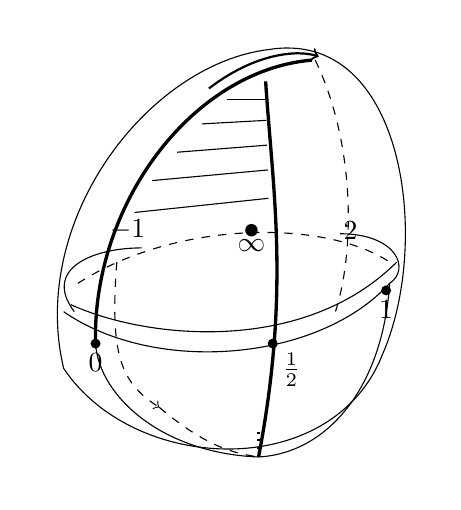
\begin{tikzpicture}[x=1cm,y=1cm,scale=.9]
\draw (0,0) .. controls (-.5,2.1) and (1.2,4.3) .. (2.9,4.5)
 .. controls (4.8,4.8) and (5.2,1.8) .. (4.5,.2)
 .. controls (3.8,-1.6) and (1,-1.5) .. (0,0);
\draw (.1,.9) .. controls (1.2,.4) and (3.4,.2) .. (4.7,1.5);
\draw (0,.8) .. controls (1.3,-.1) and (3.6,.1) .. (4.6,1.2);
\draw[dashed] (.2,1.2) .. controls (1.6,2.1) and (3.7,2.1) .. (4.6,1.5);
\draw (.15,.8) .. controls (-.3,1.4) and (.4,1.7) .. (1.1,1.7);
\draw (3.9,1.9) .. controls (4.7,1.9) and (4.9,1.4) .. (4.6,1.2);
\draw[very thick] (.45,.35) .. controls (.4,2.3) and (1.8,4.2) .. (3.5,4.35);
\draw[thick,->] (2.05,3.95) .. controls (2.7,4.45) and (3.3,4.5) .. (3.6,4.4);
\draw[very thick] (2.85,4.05) .. controls (2.95,2.5) and (3.2,1.1) .. (2.75,-1.25);
\draw[dotted,thick] (2.75,-1.25)--(2.75,-.85);
\draw[dashed,->] (.75,1.5) .. controls (.65,.2) and (.8,-.2) .. (1.35,-.55);
\draw[dashed] (1.35,-.55) .. controls (2,-1.1) and (2.4,-1.2) .. (2.75,-1.25);
\draw[dashed] (3.55,4.35) .. controls (4.15,3.1) and (4.1,1.5) .. (3.8,.7);
\draw (4.6,1.2) .. controls (4.5,-.3) and (3.7,-1.2) .. (2.75,-1.25);
\draw (.45,.35) .. controls (.5,-.4) and (1.4,-1.2) .. (2.75,-1.25);
\draw (1.0,2.2)--(2.89,2.4);
\draw (1.25,2.65)--(2.88,2.8);
\draw (1.6,3.05)--(2.87,3.15);
\draw (1.95,3.45)--(2.86,3.5);
\draw (2.3,3.8)--(2.86,3.8);
\fill (.45,.35) circle(2pt) node[below] {$0$};
\fill (2.95,.35) circle(2pt) node[below right] {$\frac12$};
\fill (4.55,1.1) circle(2pt) node[below] {$1$};
\fill (2.65,1.95) circle(2.5pt) node[below] {$\infty$};
\node at (.9,1.95) {$-1$}; \node at (4.05,1.95) {$2$};
\end{tikzpicture}}

\diagram{\begin{array}{cc}
\begin{tikzcd}[ampersand replacement=\&,row sep=small]
e_0\arrow[r,maps to]\&e_{\unsure{0|\rho}}\\
e_1\arrow[r,maps to]\&e_1-e_0
\end{tikzcd}
&
\left|\begin{tikzcd}[ampersand replacement=\&,row sep=small]
e_0\arrow[r]\&e_1\\
e_1\arrow[r]\&-e_0
\end{tikzcd}\right.
\end{array}}

\deleted{$\unsure{B|R}$}
\diagram{\begin{tikzcd}[ampersand replacement=\&,row sep=small]
e_0\arrow[r]\&e_0+e_1\\
e_1\arrow[r,maps to]\&-e_0
\end{tikzcd}}

\[
\begin{pmatrix}1&\lambda\\0&\unsure{\phi|1}\end{pmatrix}
\qquad
\begin{pmatrix}\unsure{\zeta|\lambda}&0\\0&\zeta^*\end{pmatrix}
\]

\deleted{$(\unsure{\varphi}\,\unsure{\varphi}\mathbin{-}\unsure{\tau}$}

\[
\det(u-\lambda\mathrm{id})
=\det\begin{pmatrix}1-\lambda&-1\\1&-\lambda\end{pmatrix}
\underset{\deleted{\unsure{z}}}{=}\lambda^2-\lambda+1
\]
racines sont racines primitives \unsure{6ièmes} de 1

\figure{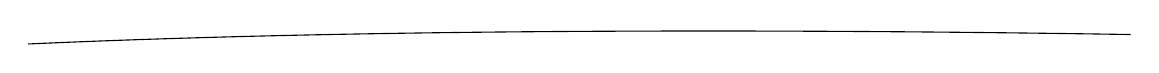
\begin{tikzpicture}[x=1cm,y=1cm]\draw (0,0) .. controls (4,.18) and (9,.2) .. (14,.12);\end{tikzpicture}}

\[
l_0\quad l_{1/2}\quad l_1\quad l_\infty
\qquad/\qquad
\dot{\sigma}_\infty,\ \unsure{\widetilde{\tau}|\widehat{\tau}},\ \sigma_\infty\tau
\]
\[
\boxed{l_\infty l_1 l_{1/2}l_0=1}
\]
\[
z\longmapsto1-z
\]
\diagram{\begin{tikzcd}[ampersand replacement=\&,row sep=small]
g:\ \mathbb P^1\arrow[r]\&\mathbb P^1\\
\infty\arrow[r,maps to]\&\infty\\
\frac12\arrow[r,maps to]\&0\\
0,1\arrow[r,maps to]\&1
\end{tikzcd}}

\[
g(z)=(2z-1)^2
\qquad
g(1-z)=(1-2z)^2.
\]
\[
(2z-\unsure{\tfrac12|\tfrac14})^2
\]

\diagram{\begin{tikzcd}[ampersand replacement=\&,row sep=small]
l_{\unsure{0|\infty}}\arrow[r,maps to]\&-1\\
l_1\arrow[r,maps to]\&+1\\
l_\infty\arrow[r,maps to,no head]\&-1
\end{tikzcd}}

\margin{102}
\scanpage{104}

CORNU\qquad Philippe\qquad 16 Juin 1978
\mspage{I}

$C_4$\quad Mathématiques

\figure{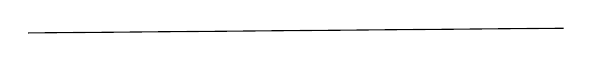
\begin{tikzpicture}[x=1cm,y=1cm]\draw (0,0)--(6.8,.06);\end{tikzpicture}}

Ces deux projections stéréographiques de l'icosaèdre (par rapport a une face et par rapport à une arête) font apparaître quelques propriétés \unsure{Combinatoire} de ce polyèdre

Par construction, on est en présence de 15 cercles distincts dont 2 ont leur centre à l'infini pour la projection par rapport a une arête, et 3 pour l'autre projection

La première constatation que l'on peut faire est que chaque cercle porte deux arêtes distinctes. (on a donc bien $2\times15=30$ arêtes.

(De meme chaque cercle porte 4 sommets, correspondant aux deux arêtes, tous distincts, chaque sommet etant le lieu d'intersection de 5 cercles on a $\dfrac{4\times15}{5}=12$ sommets. Enfin, sur chaque cercle comme on l'a vu, se trouvent 2 arêtes, de part et d'autre desquelles se trouvent une face. Chaque face etant \unsure{limité} par 3 arêtes non \unsure{cocyclique} on a
\[
\frac{4\times15}{3}=20\text{ faces.})
\]

En meme temps, l'on peut voir que l'on est aussi en présence du dodécaèdre, polyèdre dual de l'icosaèdre dont le dual est l'icosaèdre.

\margin{103}
\scanpage{105}
\mspage{\unsure{11|VI}}

\[
\lambda_0^{\unsure{\prime}}\quad\lambda_{1/2}\quad\lambda_1\quad\lambda_\infty
\]
\diagram{\begin{tikzcd}[ampersand replacement=\&]
\Pi'\arrow[r,phantom,"\subset"]\arrow[dr]\&\widehat{\Pi}_{0,3}\\
\&\widehat{\Pi}_{0,3}
\end{tikzcd}}

\figure{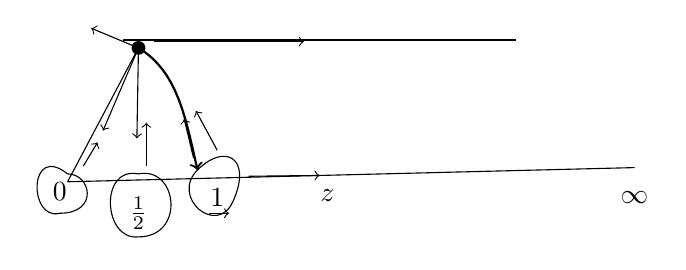
\begin{tikzpicture}[x=1cm,y=1cm]
\draw (0,0)--(7.2,.18);
\draw (.7,1.8)--(5.7,1.8);
\fill (.9,1.7) circle(2.5pt);
\draw[->] (.9,1.7)--(.45,.65);
\draw[->] (.2,.2)--(.38,.5);
\draw (.9,1.7)--(0,0);
\draw[->] (.9,1.7)--(.88,.55);
\draw[->] (1,.2)--(1,.75);
\draw[thick,->] (.9,1.7) .. controls (1.4,1.4) and (1.5,.8) .. (1.65,.15);
\draw[->] (1.6,.3)--(1.48,.8);
\draw[->] (1.9,.4)--(1.63,.9);
\draw (0,.1) .. controls (-.5,.5) and (-.5,-.5) .. (-.1,-.4)
 .. controls (.4,-.4) and (.3,.1) .. (0,.1);
\draw (.9,.1) .. controls (.4,.2) and (.45,-.75) .. (.9,-.7)
 .. controls (1.5,-.7) and (1.4,.2) .. (.9,.1);
\draw (1.65,.15) .. controls (2,.5) and (2.35,.3) .. (2.1,-.25)
 .. controls (1.9,-.7) and (1.3,-.2) .. (1.65,.15);
\draw[->] (.9,1.7)--(.3,1.95);
\draw[->] (1.1,1.78)--(3,1.78);
\draw[->] (2.3,.07)--(3.2,.08);
\draw[->] (1.8,-.4)--(2.05,-.4);
\node at (-.1,-.12) {$0$};
\node at (.9,-.4) {$\frac12$};
\node at (1.9,-.2) {$1$};
\node at (3.3,-.18) {\deleted{$\unsure{z}$}};
\node at (7.2,-.2) {$\infty$};
\end{tikzpicture}}

\[
(-2\bar j-1)^2=4\bar j^{\,2}+
\]

\diagram{\begin{tikzcd}[ampersand replacement=\&]
\lambda_{\unsure{1/2|d/2}}^{\unsure{k}}\arrow[r,"\deleted{\unsure{\zeta}}"]\&l_0
\end{tikzcd}}
\deleted{$2z-1$}\quad$\lambda$

\figure{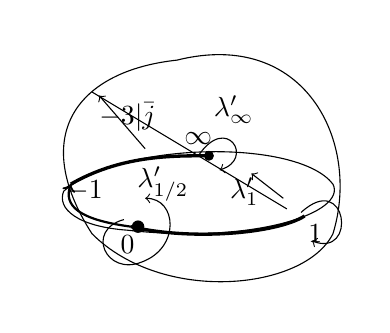
\begin{tikzpicture}[x=1cm,y=1cm,scale=.9]
\draw (0,.2) .. controls (-.9,1.6) and (-.2,2.5) .. (1.2,2.65)
 .. controls (3,3.1) and (3.8,1.5) .. (3.4,.2)
 .. controls (3,-.6) and (1,-.8) .. (0,.2);
\draw (-.4,.8) .. controls (.4,1.5) and (2.9,1.55) .. (3.4,.9)
 .. controls (3.6,.5) and (2.3,.05) .. (.5,.25)
 .. controls (-.2,.3) and (-.5,.55) .. (-.4,.8);
\draw[very thick] (.55,.3) .. controls (1.4,.1) and (2.6,.2) .. (3,.45);
\draw[thick,->] (.55,.3) .. controls (-.2,.4) and (-.4,.6) .. (-.3,.9);
\draw[very thick] (-.3,.9) .. controls (.4,1.3) and (1.1,1.3) .. (1.6,1.3);
\draw (0,2.2)--(2.75,.55);
\draw[->] (2.7,.7)--(2.25,1.05);
\draw[->] (.75,1.4)--(.1,2.15);
\fill (.65,.3) circle(2.5pt);
\fill (1.65,1.3) circle(2pt);
\draw[->] (.45,.4) .. controls (-.1,.25) and (.2,-.4) .. (.7,-.2)
 .. controls (1.25,0) and (1.2,.7) .. (.75,.7);
\draw[->] (2.95,.5) .. controls (3.6,1.1) and (3.75,-.15) .. (3.1,.1);
\draw[->] (1.5,1.3) .. controls (1.9,1.9) and (2.3,1.25) .. (1.8,1.1);
\node at (-.1,.8) {$-1$};
\node at (.5,1.85) {$-\unsure{3|\bar j}$};
\node at (1.5,1.55) {$\infty$};
\node at (.5,.05) {$0$};
\node at (3.15,.2) {$1$};
\node at (1,.9) {$\lambda'_{1/2}$};
\node at (2.15,.8) {$\lambda'_1$};
\node at (2,1.95) {$\lambda'_\infty$};
\end{tikzpicture}
\qquad
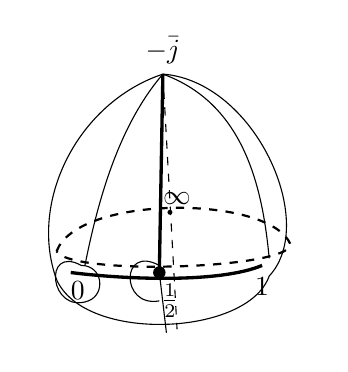
\begin{tikzpicture}[x=1cm,y=1cm,scale=.9]
\draw (0,0) .. controls (-.4,1.1) and (.3,2.5) .. (1.5,2.9)
 .. controls (2.8,2.8) and (3.7,.8) .. (3,.05)
 .. controls (2.7,-.8) and (.4,-.9) .. (0,0);
\draw[dashed,thick] (0,.4) .. controls (.3,1.2) and (3,1.2) .. (3.3,.5)
 .. controls (3.3,.15) and (.2,.05) .. (0,.4);
\draw[very thick] (.2,.1) .. controls (1,.0) and (2.3,-.05) .. (2.9,.2);
\draw[very thick] (1.5,2.9)--(1.45,.1);
\draw (.4,.2) .. controls (.6,1.2) and (.9,2.2) .. (1.5,2.9);
\draw (1.5,2.9) .. controls (2.6,2.5) and (2.9,1.4) .. (3,.3);
\draw[dashed] (1.5,2.9)--(1.7,-.7);
\draw (1.45,.1)--(1.55,-.75);
\draw (.35,.2) .. controls (-.2,.5) and (-.1,-.5) .. (.45,-.3)
 .. controls (.7,-.2) and (.65,.2) .. (.35,.2);
\draw (1.45,.2) .. controls (.9,.5) and (.9,-.4) .. (1.45,-.3);
\fill (1.45,.1) circle(2.5pt);
\fill (1.6,.95) circle(1pt);
\node[above] at (1.5,2.9) {$-\bar j$};
\node at (.3,-.15) {$0$};
\node at (2.9,-.1) {$1$};
\node at (1.6,-.3) {$\frac12$};
\node at (1.7,1.15) {$\infty$};
\end{tikzpicture}
\qquad
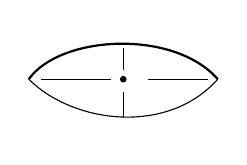
\begin{tikzpicture}[scale=.8]
\draw[thick] (0,0) .. controls (.5,.7) and (2.3,.8) .. (3,0);
\draw (0,0) .. controls (.7,-.7) and (2.2,-.9) .. (3,0);
\fill (1.5,0) circle(1.5pt);
\draw (.2,0)--(1.3,0);
\draw (1.9,0)--(2.85,0);
\draw (1.5,.15)--(1.5,.5);
\draw (1.5,-.2)--(1.5,-.6);
\end{tikzpicture}}

\deleted{$2z-1$}
\[
(2x-1+2iy)^2=(2x-1)^2-4y^2+4iy(2x-1)
\]
\[
y=0\qquad x=\tfrac12
\]

\deleted{$\dot{\sigma}_\infty(z)=1-z$}
\[
(-2\bar j+1)^2=4\bar j^{\,2}+1-4\bar j=4(\bar j^{\,2}-\bar j)
\]
\deleted{$\unsure{u}\mathbin{-}\unsure{\lambda}$}
\deleted{$\zeta^2-\zeta+1$}

\[
(2\zeta-1)^2=4\underbrace{(\zeta^2-\zeta)}_{-1}+1=-3
\]
\[
\zeta^2-\zeta+1=(\zeta-\alpha)(\zeta-\unsure{\bar\alpha|\bar\varphi})
\]
\deleted{$\alpha\mathbin{\unsure{+|\cdot}}\bar\alpha=1$}

\diagram{\begin{tikzcd}[ampersand replacement=\&]
\lambda_0\arrow[r,maps to]\&
\deleted{(l_\infty^2l_1l_0^2)^{-1}}
=l_0^{-2}l_1^{-1}l_\infty^{-2}
\end{tikzcd}}
\[
=l_0^{-1}l_\infty^{-1}=l_0^{-1}l_1l_0
\]
\diagram{\begin{array}{c}
\begin{tikzcd}[ampersand replacement=\&,row sep=small]
\lambda_{1/2}\arrow[r,maps to]\&l_0^{2\unsure{k}}\\
\lambda_1\arrow[r,maps to]\&l_1\\
\lambda_\infty\arrow[r]\&l_\infty^2
\end{tikzcd}\ \left.\vphantom{\begin{matrix}l_0^{2k}\\l_1\\l_\infty^2\end{matrix}}\right\}
\end{array}}

\deleted{$\begin{aligned}
&=(l_\infty l_0)^{-1}\\
&=\bigl(\operatorname{int}(l_0^{-1})\bigl((l_0l_\infty)^{\unsure{*}}\bigr)\bigr)^{-1}\\
&=\operatorname{int}(l_0^{-1})\bigl(\underbrace{(l_0l_\infty)^{-1}}_{l_1}\bigr)
\end{aligned}$}
\[
=\operatorname{int}(l_0^{-1})(l_1)
\]
\deleted{$l_0^{-1}l_1l_0$}
\deleted{$\begin{aligned}
l_1l_0l_\infty&=1\\
l_1^{-1}&=l_0l_\infty\\
l_1&=l_\infty^{-1}l_0^{-1}
\end{aligned}$}

\[
l_0^{-1}(l_0l_\infty\quad l_0
\]
\deleted{$ab\unsure{=}(a^{-1}b^{-1})(ba)ab$}

\margin{104}
\scanpage{106}

\begin{flushleft}
\texttt{UNIVERSITE DES SCIENCES}\\
\texttt{ET TECHNIQUES DU LANGUEDOC}

\texttt{M A T H E M A T I Q UE S}
\end{flushleft}

Montpellier, le 27 septembre 1978

Cher(e) Collègue,

Comme les années précédentes il a paru utile d'organiser au début de l'année universitaire une réunion d'information pour les étudiants des maîtrises (Math., M.A.F., Enseignement). Cette réunion aura lieu :

\begin{center}
Mardi 10 octobre 1978, à 9 h, au grand amphi.
\end{center}

A cette occasion chaque enseignant responsable d'un certificat pourra brièvement indiquer le programme et l'orientation de ce certificat. C'est dire que la présence de tous les collègues concernés est souhaitable. L'heure du 1er cours (qui pourra avoir lieu à partir de l'après-midi du mardi...) sera également rappelée à cette occasion aux étudiants.

Bien à vous,

\begin{flushright}
P. MOLINO , responsable des maîtrises Math et MAF\\
C. ROUMIEU, responsable de la maîtrise\unsure{.} enseignement
\end{flushright}

\margin{105}
\scanpage{107}
\mspage{12}

\[
\Pi'\subset\Pi_{0,3}
\]
\unsure{engendré} par

\margin{\deleted{$\unsure{\lambda_0}$}
\[
\begin{aligned}
\lambda_0&=\operatorname{int}(l_0^{-1})l_1\\
\lambda_{1/2}&=l_0^2\\
\lambda_1&=l_1\\
\lambda_\infty&=l_\infty^2.
\end{aligned}
\]}

\diagram{\begin{tikzcd}[ampersand replacement=\&,row sep=small]
\Pi_{0,3}\arrow[r]\&\{\pm1\}\arrow[r]\&1\\
l_0,l_\infty\arrow[r,maps to]\&-1\\
l_1\arrow[r,maps to]\&+1
\end{tikzcd}}

\diagram{\begin{tikzcd}[ampersand replacement=\&,column sep=small]
1\arrow[r]\&\Pi'\arrow[r,hook]\arrow[d,"\text{\unsure{épi}}"']\&
\Pi_{0,3}\arrow[r,no head]\arrow[d]\&\{\pm1\}\arrow[r,no head]\arrow[d]\&1\\
1\arrow[r]\&\Pi_{0,3}\arrow[r]\&
\Pi_{0,3}\mathbin{.}\{1,\sigma_\infty\}\arrow[r]\&\{\pm1\}\arrow[r,no head]\&1
\end{tikzcd}}

\diagram{\begin{tikzcd}[ampersand replacement=\&,row sep=small]
\lambda_0=\operatorname{int}(l_0^{-1})l_1=l_0^{-1}l_1l_0\arrow[r,maps to]\&l_0\\
\lambda_{1/2}=l_0^2\arrow[r,maps to]\&1.\\
\lambda_1=l_1\arrow[r,maps to]\&l_1\\
\lambda_\infty=l_\infty^2\arrow[r,maps to]\&l_\infty
\end{tikzcd}}
\[
l_0\longmapsto\sigma_\infty\ ?
\]

\deleted{$
\underbrace{\unsure{l_\infty^2|l_\infty^{-1}}l_1l_0^{\unsure{*}}}_{\unsure{l_\infty'|l_\infty^{-1}}}
l_0^{-1}l_1l_0
$}

\diagram{\begin{array}{c}
\widehat{\psi}:\
\boxed{\begin{tikzcd}[ampersand replacement=\&,row sep=small]
l_0\arrow[r,maps to]\&\sigma_\infty\&?\\
l_1\arrow[r,maps to]\&l_1\\
l_\infty\arrow[r,maps to]\&\varepsilon_\infty\&?
\end{tikzcd}}
\end{array}}

\[
\varepsilon_\infty l_1\sigma_\infty
=\varepsilon_\infty\varepsilon_1^2\sigma_\infty
\]

\[
\begin{aligned}
\unsure{\mathbin{-}}\,\varepsilon_0&=\sigma_\infty\rho\\
\unsure{\dot{\varepsilon}_1|\varepsilon'_1}&=\rho\sigma_\infty\\
\varepsilon_\infty&=\rho^{-1}\sigma_\infty\rho^{-1}
\end{aligned}
\]

\begin{flushright}
\texttt{MR LE PROFESSEUR GROTHENDIECK A.}\\
\texttt{MATHEMATIQUES}\qquad\texttt{5}
\end{flushright}

\[
\deleted{\rho^{-1}}\deleted{\sigma_\infty}
\deleted{\rho^{-1}}\deleted{\rho}
\deleted{\sigma_\infty}\deleted{\rho}
\sigma_\infty\sigma_\infty
\]

\margin{106}
\scanpage{108}

\begin{flushleft}
\texttt{UNIVERSITE DES SCIENCES}\\
\texttt{ET TECHNIQUES DU LANGUEDOC}\\
\texttt{--\unsure{-}--}

\uline{\textit{Service Général}} -

\textit{N° 5206}
\end{flushleft}
\begin{flushright}
MONTPELLIER, le 27 Septembre 1978

\fbox{N O T E\qquad D E\qquad S E R V I C E}
\end{flushright}

\uline{OBJET} : Collecte et livraison des bouteilles de gaz comprimé

\textit{L'important accroissement des besoins des laboratoires en gaz comprimés, rend indispensable une réorganisation du service de collecte des bouteilles de gaz comprimé et de leur livraison.}

\textit{A dater du 1er Octobre 1978, la collecte et la livraison ne se feront plus directement à chaque laboratoire mais à des points situés à proximité des portes principales d'accès de chaque bâtiment de recherche suivant le programme ci-après :}

\diagram{\begin{array}{||l|c|c||}
\hline\hline
\text{Bâtiments}&\begin{array}{c}\text{COLLECTE}\\\text{Mardi et Jeudi}\end{array}&
\begin{array}{c}\text{LIVRAISON}\\\text{Mercredi et Vendredi}\end{array}\\
\hline
\text{R.B.A. entrée principale}&\text{de 15h30 à 15h45}&\text{de 14h00 à 14h15}\\
\text{R.B.A. Ext. entrée princip.est}&\text{de 15h45 à 16h00}&\text{de 14h15 à 14h30}\\
\text{R.G. entrée principale}&\text{de 16h00 à 16h15}&\text{de 14h30 à 14h45}\\
\text{R.G. Ext. quai principal est}&\text{de 16h15 à 16h30}&\text{de 14h45 à 15h00}\\
\text{R.C. entrée principale}&\text{de 16h30 à 16h45}&\text{de 15h00 à 15h15}\\
\text{R.C. Ext. quai entrée princip.}&\text{de 16h45 à 17h00}&\text{de 15h15 à 15h30}\\
\text{R.P. entrée principale}&\text{de 17h00 à 17h15}&\text{de 15h30 à 15h45}\\
\text{R.P. Ext. quai entrée princip.}&\text{de 17h15 à 17h30}&\text{de 15h45 à 16h00}\\
\text{R.M. entrée principale}&\text{de 17h30 à 17h45}&\text{de 16h00 à 16h15}\\
\hline\hline
\end{array}}

\textit{Les utilisateurs assureront eux-mêmes le transport des bouteilles entre les laboratoires et les points de collecte et ``vice-versa''.}

\textit{Le Service Général assurera comme par le passé les transports entre l'U.S.T.L. et les fournisseurs.}

\textit{Les Chefs de laboratoires voudront bien donner toutes instructions pour que les bouteilles soient\unsure{.} rassemblées au point de collecte pour l'heure prévue.}

\begin{flushright}
LE PRESIDENT,

L Thaler

\uline{L. THALER}
\end{flushright}

\uline{Diffusion} : liste A

\margin{107}
\scanpage{109}
\mspage{13}

\diagram{\begin{tikzcd}[ampersand replacement=\&]
\widehat{\Pi}_{0,3}\arrow[r,"\widehat{\psi}_{1/2}"]\&
\widehat{\Pi}_{0,3}\mathbin{.}\{1,\sigma_\infty\}
\end{tikzcd}}

\[
\widehat{\psi}(u(x))
=\inserted{\operatorname{int}(\unsure{\mu|\psi})}u\widehat{\psi}(x)
\]

1) \quad $x=l_0$
\[
u(x)=\operatorname{int}(g_0)l_0^p
\]
\[
\widehat{\psi}(u(x))=\operatorname{int}(\widehat{\psi}(g_0))\sigma_\infty^p
\]
\[
\widehat{\psi}(x)=\sigma_\infty
\qquad u(\widehat{\psi}(x))=\sigma_\infty
\]
\[
\bigl(\operatorname{int}(\widehat{\psi}(g_0))\bigr)
\left(\underset{\substack{\Vert\\\sigma_\infty}}{\sigma_\infty^p}\right)
=\deleted{\unsure{\sigma_\infty}\operatorname{int}(g_0)}(\sigma_\infty)
\]
\deleted{d'}
\[
\boxed{\widehat{\psi}_{1/2}(g_0)=\sigma_\infty^\alpha}
\]
\margin{$\widehat{\psi}(g_0)$ commute à $\sigma_\infty$

$\alpha$ \unsure{dépend du} choix de $g_0$ mod $l_0$.}

2) \quad $x=l_1$
\[
\widehat{\psi}(u(x))
=\widehat{\psi}(\operatorname{int}(g_1)l_1^p)
=\operatorname{int}(\widehat{\psi}(g_1))(l_1^p)
\]
\[
u(\widehat{\psi}(x))=u(l_1)=\operatorname{int}(g_1)(l_1^p)
\]
\[
\boxed{\widehat{\psi}_{1/2}(g_1)=g_1l_1^\beta}
\]

\margin{\[
g_1=g\rho(g_0)=\sigma_\infty(g_0l_0^\gamma)
=\sigma_\infty(g_0)l_1^\gamma
\]}

\[
\widehat{\psi}\bigl(\sigma_\infty(g_0)l_1^\gamma\bigr)
=\sigma_\infty(g_0)l_1^{\beta+\gamma}
\]
\[
\boxed{\widehat{\psi}_{1/2}(\sigma_\infty(g_0))
=\sigma_\infty(g_0)l_1^\beta}
\]
\[
\sigma_\infty(g_0)^{-1}g_0=h_0
\qquad
\sigma_\infty(g_0)=g_0h_0^{-1}
\]
\margin{$\beta$ \unsure{ne dépend pas du choix} de $g_0$ mod $L_0$}
\[
\widehat{\psi}(g_0h_0^{-1}l_1^\gamma)
=\deleted{\sigma_\infty(g_0)}g_0h_0^{-1}l_1^{\beta+\gamma}
\]
\[
\underbrace{\widehat{\psi}(g_0)}_{\sigma_\infty^\alpha}
\widehat{\psi}(h_0^{-1})\deleted{l_1^\gamma}
=g_0h_0^{-1}l_1^{\beta+\deleted{\gamma}}
\]
\[
\widehat{\psi}(h_0)=l_1^{-\beta}h_0g_0^{-1}\sigma_\infty^\alpha
\]

$\bigl[$3) \quad $x=l_\infty$
\[
\widehat{\psi}(u(x))
=\widehat{\psi}(\operatorname{int}(g_\infty)l_\infty^p)
=\operatorname{int}(\widehat{\psi}(g_\infty))\varepsilon_\infty^p
\]
\[
u\widehat{\psi}(x)=u(\varepsilon_\infty)
=\operatorname{int}(g_\infty)\varepsilon_\infty^p
\]
\[
\deleted{\unsure{\operatorname{int}}}\widehat{\psi}(g_\infty)=g_\infty
\]

\margin{108}
\scanpage{110}

\begin{flushleft}
\texttt{UNIVERSITE DES SCIENCES}\\
\texttt{ET}\\
\texttt{TECHNIQUES DU LANGUEDOC}

\rule{3cm}{.3pt}

Service du Personnel

\rule{1cm}{.3pt}

AMC/MM

\textit{Diffusion Générale + Affichage}

n° 4713
\end{flushleft}

\begin{flushright}
\texttt{MR LE PROFESSEUR GROTHENDIECK A.}\\
\texttt{MATHEMATIQUES}\qquad\texttt{5}
\end{flushright}

\begin{center}
\uline{N O T E\qquad D' I N F O R M A T I O N}
\end{center}

J'ai l'honneur de vous faire connaître que la validité des laissez-passer provisoires \textit{(bristol jaune)} délivrés au titre de l'année universitaire 1977-1978, expirera le \uline{31 Octobre 1978}.

En conséquence, les détenteurs de ces cartes d'accès au Campus de l'Université sont invités à se présenter au Service du Personnel, \textit{Bureau d'Accueil}, munis d'une attestation de leur chef de service et de leur carte grise, pour retirer les nouveaux laissez-passer établis pour l'année universitaire 1978-1979.

Je rappelle qu'outre les personnels de l'Enseignement Supérieur et de l'Administration de l'Université des Sciences et Techniques du Languedoc, sont susceptibles d'avoir accès à l'intérieur de l'Etablissement avec leur véhicule :

\begin{itemize}
\item[-] le Personnel du C.N.R.S.,
\item[-] le Personnel sous convention,
\item[-] Les Thésards (d'Etat, de 3ème cycle, et d'Université, qui devront fournir, en lieu et place de l'attestation, un certificat de scolarité
\end{itemize}

\begin{flushright}
\inserted{\unsure{p.c.|p.o.}} Le Président,

\unsure{Y. Pietrasanta}
\end{flushright}

\margin{109}
\scanpage{111}
\mspage{14}

\diagram{\begin{tikzcd}[ampersand replacement=\&,row sep=small]
\Pi'\arrow[r]\&\pm1\\
\lambda_0,\lambda_{1/2},\lambda_1,\lambda_\infty\arrow[r,maps to]\&-1
\end{tikzcd}}

\diagram{\begin{tikzcd}[ampersand replacement=\&]
\Pi_{0,3}\arrow[r]\&\mathbb Z/4\mathbb Z
\end{tikzcd}}

\diagram{\begin{array}{r|l}
\unsure{\lambda}\ l_0^{-1}l_1l_0\ \longrightarrow&\\
l_0^2&\longmapsto2\ \mathrm{mod}\ 4\\
l_1&\\
l_\infty^2&
\end{array}}

\diagram{\begin{tikzcd}[ampersand replacement=\&,row sep=small]
l_0\arrow[r,maps to]\&\alpha_0\\
l_1\arrow[r,maps to]\&\alpha_1=2\ \mathrm{mod}\ 4
\end{tikzcd}}
\[
l_\infty=\alpha_\infty=
\]
\[
\begin{aligned}
\alpha_0+\alpha_\infty&\equiv2&&(4)\\
2\alpha_0&\equiv2&&(4)\\
2\alpha_\infty&\equiv2&&(\unsure{4|n})\\
\alpha_0&\equiv\pm1&&(4)\\
\alpha_\infty&\equiv\pm1&&(4)
\end{aligned}
\]

\diagram{\begin{array}{c}
\boxed{\begin{tikzcd}[ampersand replacement=\&,row sep=small]
l_0,l_\infty\arrow[r,maps to]\&1\ \mathrm{mod}\ 4\\
l_1\arrow[r,maps to]\&2\ \mathrm{mod}\ 4
\end{tikzcd}}
\end{array}}

\unsure{sps}\quad $\alpha_0\equiv1$

alors\quad $\alpha_\infty\equiv1$

\diagram{\begin{tikzcd}[ampersand replacement=\&,column sep=small]
1\arrow[r,no head]\&\Pi''\arrow[r]\arrow[dr]\&
\Pi_{0,3}\arrow[r]\&\mathbb Z/4\mathbb Z\arrow[r,no head]\&1\\
\&\deleted{\unsure{\lambda_0^2}\mathbin{.}\triangleleft\Pi''_{\unsure{\infty}}}\&
\displaystyle\Pi''/\Delta\left(
\underset{\substack{\Vert\\l_0^{-1}l_1^2l_0}}{\unsure{l_0^2|\lambda_0^2}},
\underset{\substack{\Vert\\l_1^2}}{\lambda_1^2},
\underset{\substack{\Vert\\l_\infty^4}}{\lambda_\infty^2}
\right)
\end{tikzcd}}

\deleted{\unsure{A.} Grothendieck}

\diagram{\begin{tikzcd}[ampersand replacement=\&,column sep=small]
\&\operatorname{Aut\,ext}_{\unsure{C_\infty|\mathrm{co}}}(\Pi'')'\\
1\arrow[r]\&\widehat{\unsure{\mathcal G|\mathfrak S}}_{0,3}^{+}\arrow[u]\arrow[r]\&
\mathcal M_{0,3}\arrow[r,"\unsure{l_0^2}"]\arrow[d]\&
\unsure{\mathbb{\Gamma}|\Gamma}\arrow[r,no head]\&1\\
\&\&N'_{1,1}
\end{tikzcd}}

\margin{110}
\scanpage{112}

\begin{flushleft}
\textbf{UNIVERSITE DES SCIENCES ET TECHNIQUES}\\
\textbf{DU LANGUEDOC}

\rule{.6cm}{.3pt}

\textbf{INSTITUT DE MATHEMATIQUES}\\
\textbf{Place Eugène Bataillon}\\
\textbf{34060 MONTPELLIER CEDEX}

\rule{.8cm}{.3pt}
\end{flushleft}

\begin{flushright}
Montpellier, le 26 septembre 1978

Note d'Information reçue\\
du Secrétariat de\\
l'U.S.T.L.
\end{flushright}

La date du 10 octobre pour la soutenance du rapport de stage est une date impérative.

S'il y a un cas particulier (raison valable) il est possible de demander une dérogation au Président (en fait, c'est M. NOUAZE qui s'occupe de cela).

Il n'est pas possible de transformer une inscription en cours d'année. Si l'étudiant se réinscrit en D.E.A. pour soutenir son rapport de stage un peu plus tard, la Scolarité considère qu'il a soutenu son rapport à la session de juin 1979. Donc, l'étudiant perd une année.

\begin{flushright}
N. ROBY
\end{flushright}

\figure{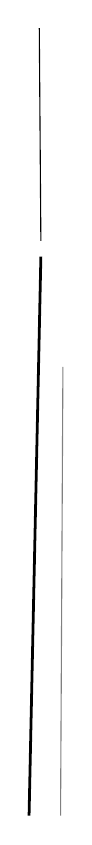
\begin{tikzpicture}
\draw (0,0)--(.02,-2.7);
\draw[line width=1pt] (.02,-2.9)--(-.13,-10);
\draw[thin,gray] (.3,-4.3)--(.27,-10);
\end{tikzpicture}}

\margin{111}
\scanpage{113}
\figure{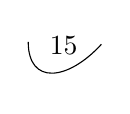
\begin{tikzpicture}[x=1cm,y=1cm]
\node at (0,0) {\mspage{15}};
\draw (-.45,.05) .. controls (-.45,-.5) and (.05,-.45) .. (.48,.02);
\end{tikzpicture}}

\diagram{\begin{tikzcd}[ampersand replacement=\&,row sep=small]
l_0^{-1}l_1l_0=\lambda_0\arrow[r,maps to]\&1\\
l_0^2=\lambda_{1/2}\arrow[r]\&l_0\\
l_1=\lambda_1\arrow[r,no head]\&l_1\\
l_\infty^2=\lambda_\infty\arrow[r,no head]\&l_\infty
\end{tikzcd}
\qquad
\begin{tikzcd}[ampersand replacement=\&,row sep=small]
l_0\arrow[r,maps to,no head]\&\varepsilon_0\\
l_1\arrow[r,maps to,no head]\&l_1\\
l_\infty\arrow[r,no head]\&\varepsilon_\infty
\end{tikzcd}}

\[
\varepsilon_\infty l_1\varepsilon_0=1
\qquad\text{i.e.}\qquad
\underbrace{\rho^{-1}\sigma_\infty\deleted{\rho^{-1}}}
\underbrace{\deleted{\rho}\deleted{\sigma_\infty}
\deleted{\rho}\deleted{\sigma_\infty}}
\deleted{\sigma_\infty}\deleted{\rho}
=\rho^{-1}\sigma_\infty
\]

\[
\begin{aligned}
\varepsilon_0&=\sigma_\infty\rho\\
\unsure{\varepsilon_1|l_1}&=\rho\sigma_\infty\\
\varepsilon_\infty&=\rho^{-1}\sigma_\infty\rho^{-1}
\end{aligned}
\]

\margin{112}
\scanpage{114}

CORNU\qquad Ph\qquad 16/06/78
\mspage{$\overline{\text{\uline{VI}}}$}

C4.Math

\figure{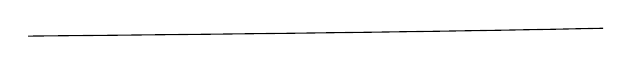
\begin{tikzpicture}[x=1cm,y=1cm]\draw (0,0) .. controls (2,.02) and (5,.05) .. (7.3,.1);\end{tikzpicture}}

Si l'on \unsure{associ} à chaque trièdre, une Couleur, on obtient ainsi un coloriage des arêtes de l'icosaèdre, tel que deux arêtes distinctes ayant la meme Couleur, \deleted{\unsure{ne} \unsure{se}} n'ont jamais de Sommets en Commun.

En relation avec tout ça, il aurait fallu parler ; du groupe des automorphismes de l'icosaèdre, dont le neutre et l'antipodisme Constituent le Centre.

\deleted{\unsure{ordre}}

\begin{center}
\uline{\unsure{Cornu}}.
\end{center}

\margin{113}
\scanpage{115}
\mspage{16}

\diagram{\begin{tikzcd}[ampersand replacement=\&,row sep=small]
\lambda_0=l_0^{-1}l_1l_0\arrow[r,maps to]\&l_{\unsure{1|0}}\\
\lambda_{1/2}=l_0^2\arrow[r,maps to]\&l_\infty\\
\lambda_1=l_1\arrow[r,maps to,no head]\&l_0\\
\lambda_\infty=l_\infty^2\arrow[r,maps to]\&\unsure{\phi|1}
\end{tikzcd}
\qquad
\begin{tikzcd}[ampersand replacement=\&,row sep=small]
l_0\arrow[r,maps to,no head]\&\varepsilon_\infty\\
l_1\arrow[r,maps to,no head]\&l_0\\
l_\infty^{\deleted{\unsure{2}}}\arrow[r]\&\sigma_\infty
\end{tikzcd}}

\[
(l_1\varepsilon_0)^{-1}
=(\rho\sigma_\infty\deleted{\rho}\deleted{\sigma_\infty}
\deleted{\sigma_\infty}\deleted{\rho})^{-1}
=\sigma_\infty\rho^{-1}
\]
\[
(l_0\varepsilon_\infty)^{-1}
=(\sigma_\infty\deleted{\rho}\deleted{\sigma_\infty}
\deleted{\rho}\deleted{\rho^{-1}}\deleted{\sigma_\infty}
\deleted{\rho^{-1}})=\sigma_\infty
\]

\diagram{\begin{tikzcd}[ampersand replacement=\&]
\widehat{\psi}_\infty:\quad\widehat{\Pi}_{0,3}\arrow[r]\&
\widehat{\Pi}_{0,3}\mathbin{.}\{1,\sigma_\infty\}
\end{tikzcd}}

\[
\widehat{\psi}_\infty
\]

\diagram{\begin{tikzcd}[ampersand replacement=\&]
\mathrm{Sl}(2,12)'\simeq
\bigl(\mathrm{Sl}(2,\mathbb Z/4)\times
\mathrm{Sl}(\unsure{0|2},\mathbb Z/3)\bigr)/\pm1
\arrow[d]\\
\unsure{\mathcal G_3|\mathfrak S_3}\simeq\mathrm{Sl}(2,\mathbb Z/2)
\end{tikzcd}}

\diagram{\begin{tikzcd}[ampersand replacement=\&]
\widehat{\unsure{\mathcal G|\mathfrak S}}_{0,3}^{+}\arrow[d]\\
\mathrm{Sl}(2,\widehat{\mathbb Z})'\arrow[r]\arrow[d,equals]\&
\mathrm{Sl}(\unsure{0|2},\mathbb Z/12\mathbb Z)\arrow[r]\&1\\
\deleted{\widehat{\unsure{\mathcal G|\mathfrak S}}_{0,3}^{+}}
\end{tikzcd}}

\deleted{$
\begin{array}{c|ccl}
(c,d)&c\equiv0\ (3)&D=d^2\in\{0,1\}\deleted{\unsure{2|1}}&
0\ \text{\unsure{exclus|exclu}}\\
&c\equiv1\ (3)&D=1+d^2+d=\deleted{\unsure{d}}\in\{1,0\}&
0\ \text{\unsure{exclus|exclu}}\\
&c\equiv-1\ (3)&D=1+d^2-d\in\{1,0\}&
0\ \text{\unsure{inclus}}
\end{array}
$}\quad !!!

\margin{114}
\scanpage{116}

CORNU\qquad Ph.\qquad 16/06/78
\mspage{\uline{V}}

C4.Math

\figure{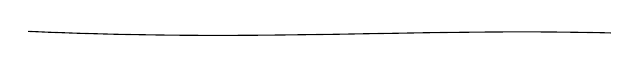
\begin{tikzpicture}[x=1cm,y=1cm]\draw (0,0) .. controls (3,-.13) and (5,.04) .. (7.4,-.02);\end{tikzpicture}}

On peut définir ainsi
\diagram{\begin{tikzcd}[ampersand replacement=\&,row sep=small]
\rho:\quad A\arrow[r]\&A\\
a\arrow[r,maps to]\&\rho(a)
\end{tikzcd}}
avec
\[
a\in C_a\longrightarrow\rho(a)\in\rho'(C_a)
\]

Donc Notons \deleted{\illegible{1}}
\[
\bar A=A/(\underline a)\simeq\mathcal C
\]

$\bar A$ se décompose en 5 ``paquets'' de 3 ``cercles''

On appelle chaque paquet un trièdre, Soit $\mathcal T$ l'ensemble des trièdres.

On a donc l'isomorphisme $\mathcal T\simeq\bar A/(\rho)$

ou $\bar A/(\rho)$ désigne l'ensemble des classes, d'éléments de $\bar A$, modulo $\rho$.

On dira que deux arêtes sont orthogonales si elles sont distinctes et si elles appartiennent à la meme orbite sous $\rho$

\uline{\unsure{ie}}
\[
a_1\perp a_{\unsure{2|1}}
\Longleftrightarrow
a_1=\rho(a_2)\quad\text{ou}\quad a_1=\rho^{-1}(a_2)
\]

On remarque que si deux arêtes sont orthogonales elles n'ont pas de Sommets en Commun

Notons $A(s)$ l'ensemble des arêtes issues de $s$.

On a $A(s)\xrightarrow{\sim}\mathcal T$.

En effet on a $|A(s)|=|\mathcal T|=5$

D'autre part si deux arêtes \deleted{sont} distinctes sont dans $A(s)$, elles ont un sommet en commun, $\uline{s}$, et donc elles n'appartiennent pas au meme trièdre $\Rightarrow$ injectivité

On a bien une bijection

\margin{115}
\scanpage{117}

\begin{flushright}
Calculs divers\\
sur Teichmüller

\medskip
Lettre Deligne sur\\
groupes profinis
\end{flushright}

\margin{116}
\scanpage{118}

\begin{flushright}
27/3/81
\end{flushright}

Cher Schurik,

Je n'ai pas de référence à proposer pour les pro-groupes libres, et l'essentiel de ce que je connais vient du Ch I de Serre, Cohomologie Galoisienne [cité CG]

On a

-- un sous-groupe d'un groupe libre est libre

\quad (clair par l'interprétation libre $\Longleftrightarrow\pi_1$ (un CW complexe de dim 1)

-- on comprend assez bien les pro-p-groupes libres, voire même les groupes nilpotents libres (?)

\margin{\figure{\begin{tikzpicture}[x=1cm,y=1cm]\draw[->] (0,.35) .. controls (.1,.15) and (.22,.05) .. (.25,0);\end{tikzpicture}}
voir CG, I5-I8 et références à Lazard}

et ces deux remarques doivent suffire pour tes questions sur ``centre'' et ``ordre fini''

a) si $u\in\hat L$ est d'ordre fini, soit $H\subset\hat L$ distingué ouvert ne contenant pas $u$\unsure{$\overset{\circ}{!}$}.
\margin{(mieux : $H\cap\mathbb Zu=\{e\}$)}
Remplaçant $L$ par $L\cap(H.\mathbb Zu)$, on se ramène à supposer \deleted{que} l'existence de
\[
L\overset{\varphi}{\twoheadrightarrow}\mathbb Z/n\mathbb Z
\quad\text{tel que }1\in\mathbb Z/n\mathbb Z\text{ puisse se relever}
\]
en un élément d'ordre $n$ \inserted{de $\hat L$}. Ceci est déjà faux avec $L$ remplacé par $L/(L,L)$.
\[
[(,)\text{ commutateurs}]
\]

b) pour $u\in\hat L$ central, on se ramène de même à supposer qu'on a
\[
L\overset{\varphi}{\twoheadrightarrow}\mathbb Z/n\mathbb Z,\quad
\varphi(u)\ne0,
\]
et une contradiction en regardant ce que serait l'image de \deleted{\unsure{$L$}} $u$ dans
\[
L/(\operatorname{Ker}\varphi,\operatorname{Ker}\varphi)
\qquad
\text{(et l'action de }u\text{ sur }
\operatorname{Ker}\varphi/(\operatorname{Ker}\varphi,\operatorname{Ker}\varphi))
\]

\margin{118}
\scanpage{119}

Que le centre de tout sous-groupe d'indice fini de $\operatorname{Gal}(\overline{\mathbb Q}/\mathbb Q)$ soit trivial doit pouvoir se déduire de même de ce qu'on comprend bien les extensions abéliennes : pour $L/K$ cyclique, $\operatorname{Gal}(L/K)$ de générateur $\sigma$, et $K/\mathbb Q$ fini, $\sigma$ agit non trivialement sur $\operatorname{Gal}(L^{ab}/L)$, $L^{ab}$ extension abélienne maximale de $L$, car
\[
\operatorname{Gal}(L^{ab}/L)=
\pi_0(\text{groupe des \deleted{\unsure{gr}} classes d'idèles de }L)
\]
qu'on comprend. Par exemple, si $p$ se décompose complètement dans $L$ ($p$ idéal de $K\longmapsto p_1\cdots p_g$ au-dessus dans $L$), il existe une extension abélienne de $L$ ramifiée en un des $p_i$, et pas en les autres, alors que $\operatorname{Gal}(L/K)$ permute les $p_i$

On sait maintenant que tout sous-groupe fini de Teichmuller correspond bien à un groupe fini d'automorphismes d'une courbe convenable. Je devrais demander à A'Campo pour une référence, s'il en existe déjà. Si je me rappelle bien, on montre que pour une métrique (finslérienne) \deleted{\unsure{ca}} naturelle convenable, l'espace de Teichmuller est ``\deleted{\unsure{en}} négativement courbé'' en un sens qui permette\deleted{\unsure{nt}} de prouver à l'imitation de E. Cartan que tout groupe compact d'isométries a un point-fixe.

\margin{J'ai demandé à Poenaru : référence : Kerchof, dans Bull AMS, il y a moins de 2 ans. Il emploie la théorie de Teichmüller, revue par Thurston.
\figure{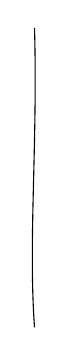
\begin{tikzpicture}[x=1cm,y=1cm]\draw (0,0) .. controls (.04,-1.5) and (-.08,-2.7) .. (0,-3.8);\end{tikzpicture}}}

Я женатый с сентября, а Лена приехала только месяц назад : она приехала (в Брюсселе) 3\textsuperscript{e} марта. Всё новое для \unsure{неё}. Мне сказала : ``Нечего \unsure{автоматическо|автоматически} ; мне всегда надо думать. Это очень интересно, а я иногда \unsure{устаюсь}''.

Il y aurait plus à raconter que ne me le permet mon russe, ou le bas de cette page.

\begin{center}
Bien à toi\\
\hfill Pierre
\end{center}

\margin{119}
\scanpage{120}

Cher Schurik,

Voici déjà le fascicule de résultat sur le corps de classes. Pour le corps de classe lui-même, une référence concise est le § 1 de

Tate -- Number theoretic background --\qquad Proc. of Symposia in Pure Math. \uline{33} (79)

\hfill AMS

p 3-26\hfill (Corvallis, vol 2)

\quad (§ 1 = 3-9)

On a

\uline{Local}

$K$ corps local
\[
\operatorname{Gal}(\bar K/K)^{ab}=\hat K^*,\quad\text{ou mieux}
\]
\[
W(\bar K/K)^{ab},\quad
\text{ou }W(\bar K/K):=\text{le sous-gr de }\operatorname{Gal}(\bar K/K)\text{ qui}
\]
induit sur le corps résiduel une puissance entière de Frobenius
\[
=K^*
\]

\diagram{\begin{tikzcd}[ampersand replacement=\&,column sep=large,row sep=huge]
W(\bar K/K)\arrow[r]\arrow[d,"{\substack{\text{quelle puissance}\\\text{de }F\text{ géométrique sur}\\\text{le corps résiduel}}}"']
\& K^*\arrow[d,"\text{valuation}"]\\
\mathbb Z\arrow[r,equal]\&\mathbb Z
\end{tikzcd}}

$L/K$ fini :
\diagram{\begin{tikzcd}[ampersand replacement=\&,column sep=large,row sep=large]
W(\bar K/K)^{ab}\arrow[r,equal]\arrow[d,"\text{transfert}"]
\& K^*\arrow[d,hook]\\
W(\bar K/L)^{ab}\arrow[r,equal]\&L^*
\end{tikzcd}}
\diagram{\begin{tikzcd}[ampersand replacement=\&,column sep=large,row sep=large]
W(\bar K/K)\arrow[r]\& K^*\\
W(\bar K/L)\arrow[u,hook]\arrow[r]\&L^*\arrow[u,"N"']
\end{tikzcd}}

\uline{Global}

$K$ corps global -- même énoncés en remplaçant $K^*$ du cas local par le groupe des classes d'idèles $\mathbb A^*/K^*$ -- Plutôt :

\figure{
\begin{tikzpicture}
\node[anchor=west] at (0,0) {corps de fonctions :};
\draw[dashed] (0,-.23)--(3.1,-.23);
\end{tikzpicture}}

\diagram{\begin{tikzcd}[ampersand replacement=\&,column sep=huge,row sep=huge]
W(\bar K/K)^{ab}\arrow[r,leftrightarrow]\arrow[d,"{\substack{\text{effet sur la clot alg}\\\text{du corps des constantes}}}"']
\&\mathbb A^*/K^*\arrow[d,"{\log_q\unsure{\lVert\ \rVert|\lvert\ \rvert}}"]\\
\mathbb Z\arrow[r,equal]\&\mathbb Z
\end{tikzcd}}

\margin{120}
\scanpage{121}

\figure{
\begin{tikzpicture}
\node[anchor=west] at (0,0) {corps de \# :};
\draw[dashed] (0,-.25)--(2.1,-.25);
\end{tikzpicture}}

\[
\operatorname{Gal}(\bar K/K)^{ab}
\longleftrightarrow
\pi_0(\mathbb A^*/K^*)=\text{limite projective des}
\]
$U\backslash\mathbb A^*/K^*$ pour $U$ sous-groupe ouvert d'indice fini de
\[
\prod_{v\mid\infty}K_v^*\times
\prod_{v\nmid\infty}O_v^*
\]

(pour
\[
U=
\prod_{v\text{ réel}}\mathbb R^{+*}
\times\prod_{v\text{ complexe}}\mathbb C^*
\times\prod_{v\nmid\infty,\ v\notin S}O_v^*
\times\prod_{v\in S}(1+m_v^{f_v})^*,
\]
ce quotient est le groupe des $\prod m_v^{f_v}$-classes d'idéaux stricts : le groupe des idéaux premiers à $S$, avec l'équivalence $a\sim b$ si $a=\alpha b$ avec $\alpha\in K^*$, $S$-entier, positif aux places réelles, $\alpha\equiv1\ (m_v^{f_v})\quad\forall v\in S$)

Il est souvent utile de savoir que, d'après Chevalley, tout sous-groupe d'indice fini du groupe des $S$-unités $H^0(\operatorname{Spec}O-S,O^*)$ \deleted{contient} contient un sous-groupe défini par une condition de congruence : $x\equiv1\ (b)$, $b$ idéal $\ne0$ convenable.

\uline{Local-global}

\diagram{\begin{tikzcd}[ampersand replacement=\&,column sep=huge,row sep=large]
\operatorname{Gal}(\bar K_v/K_v)^{ab}
\arrow[d,"{\substack{\text{groupe de}\\\text{décomposition}}}"']
\&K_v^*\arrow[l]\arrow[d]\\
\operatorname{Gal}(\bar K/K)^{ab}
\&\mathbb A^*/K^*\arrow[l]
\end{tikzcd}}

\begin{center}
\figure{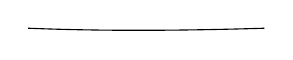
\begin{tikzpicture}[x=1cm,y=1cm]\draw (0,0) .. controls (1,-.04) and (2,-.03) .. (3,0);\end{tikzpicture}}
\end{center}

Pour la multiplication complexe, le théorème fondamental est celui de Shimura et Taniyama. Voici la façon de l'énoncer que je préfère (sauf qu'on ne parle pas assez de motifs).

Soit : $K$ un corps extension quadratique totalement imaginaire d'un corps de nombres totalement réel $F$.
\[
\unsure{g|q}=[F:\mathbb Q]
\]

\margin{121}
